\documentclass[twoside]{book}

% Packages required by doxygen
\usepackage{calc}
\usepackage{doxygen}
\usepackage{graphicx}
\usepackage[utf8]{inputenc}
\usepackage{makeidx}
\usepackage{multicol}
\usepackage{multirow}
\usepackage{textcomp}
\usepackage[table]{xcolor}

% Font selection
\usepackage[T1]{fontenc}
\usepackage{mathptmx}
\usepackage[scaled=.90]{helvet}
\usepackage{courier}
\usepackage{amssymb}
\usepackage{sectsty}
\renewcommand{\familydefault}{\sfdefault}
\allsectionsfont{%
  \fontseries{bc}\selectfont%
  \color{darkgray}%
}
\renewcommand{\DoxyLabelFont}{%
  \fontseries{bc}\selectfont%
  \color{darkgray}%
}

% Page & text layout
\usepackage{geometry}
\geometry{%
  a4paper,%
  top=2.5cm,%
  bottom=2.5cm,%
  left=2.5cm,%
  right=2.5cm%
}
\tolerance=750
\hfuzz=15pt
\hbadness=750
\setlength{\emergencystretch}{15pt}
\setlength{\parindent}{0cm}
\setlength{\parskip}{0.2cm}
\makeatletter
\renewcommand{\paragraph}{%
  \@startsection{paragraph}{4}{0ex}{-1.0ex}{1.0ex}{%
    \normalfont\normalsize\bfseries\SS@parafont%
  }%
}
\renewcommand{\subparagraph}{%
  \@startsection{subparagraph}{5}{0ex}{-1.0ex}{1.0ex}{%
    \normalfont\normalsize\bfseries\SS@subparafont%
  }%
}
\makeatother

% Headers & footers
\usepackage{fancyhdr}
\pagestyle{fancyplain}
\fancyhead[LE]{\fancyplain{}{\bfseries\thepage}}
\fancyhead[CE]{\fancyplain{}{}}
\fancyhead[RE]{\fancyplain{}{\bfseries\leftmark}}
\fancyhead[LO]{\fancyplain{}{\bfseries\rightmark}}
\fancyhead[CO]{\fancyplain{}{}}
\fancyhead[RO]{\fancyplain{}{\bfseries\thepage}}
\fancyfoot[LE]{\fancyplain{}{}}
\fancyfoot[CE]{\fancyplain{}{}}
\fancyfoot[RE]{\fancyplain{}{\bfseries\scriptsize Generated on Tue Dec 17 2013 13\-:49\-:23 for P6\-\_\-\-L\-D\-H by Doxygen }}
\fancyfoot[LO]{\fancyplain{}{\bfseries\scriptsize Generated on Tue Dec 17 2013 13\-:49\-:23 for P6\-\_\-\-L\-D\-H by Doxygen }}
\fancyfoot[CO]{\fancyplain{}{}}
\fancyfoot[RO]{\fancyplain{}{}}
\renewcommand{\footrulewidth}{0.4pt}
\renewcommand{\chaptermark}[1]{%
  \markboth{#1}{}%
}
\renewcommand{\sectionmark}[1]{%
  \markright{\thesection\ #1}%
}

% Indices & bibliography
\usepackage{natbib}
\usepackage[titles]{tocloft}
\setcounter{tocdepth}{3}
\setcounter{secnumdepth}{5}
\makeindex

% Hyperlinks (required, but should be loaded last)
\usepackage{ifpdf}
\ifpdf
  \usepackage[pdftex,pagebackref=true]{hyperref}
\else
  \usepackage[ps2pdf,pagebackref=true]{hyperref}
\fi
\hypersetup{%
  colorlinks=true,%
  linkcolor=blue,%
  citecolor=blue,%
  unicode%
}

% Custom commands
\newcommand{\clearemptydoublepage}{%
  \newpage{\pagestyle{empty}\cleardoublepage}%
}


%===== C O N T E N T S =====

\begin{document}

% Titlepage & ToC
\hypersetup{pageanchor=false}
\pagenumbering{roman}
\begin{titlepage}
\vspace*{7cm}
\begin{center}%
{\Large P6\-\_\-\-L\-D\-H \\[1ex]\large 1.\-0 }\\
\vspace*{1cm}
{\large Generated by Doxygen 1.8.5}\\
\vspace*{0.5cm}
{\small Tue Dec 17 2013 13:49:23}\\
\end{center}
\end{titlepage}
\clearemptydoublepage
\tableofcontents
\clearemptydoublepage
\pagenumbering{arabic}
\hypersetup{pageanchor=true}

%--- Begin generated contents ---
\chapter{R\-E\-A\-D\-M\-E}
\label{md__r_e_a_d_m_e}
\hypertarget{md__r_e_a_d_m_e}{}
\hyperlink{class_dijkstra}{Dijkstra} Algorithm 
\chapter{Namespace Index}
\section{Packages}
Here are the packages with brief descriptions (if available)\-:\begin{DoxyCompactList}
\item\contentsline{section}{\hyperlink{namespacemain}{main} }{\pageref{namespacemain}}{}
\item\contentsline{section}{\hyperlink{namespacemain_1_1java}{main.\-java} }{\pageref{namespacemain_1_1java}}{}
\item\contentsline{section}{\hyperlink{namespacemain_1_1java_1_1com}{main.\-java.\-com} }{\pageref{namespacemain_1_1java_1_1com}}{}
\item\contentsline{section}{\hyperlink{namespacemain_1_1java_1_1com_1_1company}{main.\-java.\-com.\-company} }{\pageref{namespacemain_1_1java_1_1com_1_1company}}{}
\item\contentsline{section}{\hyperlink{namespacemain_1_1java_1_1com_1_1company_1_1dijkstratest}{main.\-java.\-com.\-company.\-dijkstratest} }{\pageref{namespacemain_1_1java_1_1com_1_1company_1_1dijkstratest}}{}
\item\contentsline{section}{\hyperlink{namespacetest}{test} }{\pageref{namespacetest}}{}
\item\contentsline{section}{\hyperlink{namespacetest_1_1java}{test.\-java} }{\pageref{namespacetest_1_1java}}{}
\item\contentsline{section}{\hyperlink{namespacetest_1_1java_1_1com}{test.\-java.\-com} }{\pageref{namespacetest_1_1java_1_1com}}{}
\item\contentsline{section}{\hyperlink{namespacetest_1_1java_1_1com_1_1company}{test.\-java.\-com.\-company} }{\pageref{namespacetest_1_1java_1_1com_1_1company}}{}
\item\contentsline{section}{\hyperlink{namespacetest_1_1java_1_1com_1_1company_1_1dijkstratest}{test.\-java.\-com.\-company.\-dijkstratest} }{\pageref{namespacetest_1_1java_1_1com_1_1company_1_1dijkstratest}}{}
\end{DoxyCompactList}

\chapter{Hierarchical Index}
\section{Class Hierarchy}
This inheritance list is sorted roughly, but not completely, alphabetically\-:\begin{DoxyCompactList}
\item \contentsline{section}{main.\-java.\-com.\-company.\-dijkstratest.\-Community}{\pageref{classmain_1_1java_1_1com_1_1company_1_1dijkstratest_1_1_community}}{}
\item Comparable\begin{DoxyCompactList}
\item \contentsline{section}{main.\-java.\-com.\-company.\-dijkstratest.\-Pair}{\pageref{classmain_1_1java_1_1com_1_1company_1_1dijkstratest_1_1_pair}}{}
\item \contentsline{section}{main.\-java.\-com.\-company.\-dijkstratest.\-Vertex}{\pageref{classmain_1_1java_1_1com_1_1company_1_1dijkstratest_1_1_vertex}}{}
\end{DoxyCompactList}
\item \contentsline{section}{main.\-java.\-com.\-company.\-dijkstratest.\-Connection\-Matrix}{\pageref{classmain_1_1java_1_1com_1_1company_1_1dijkstratest_1_1_connection_matrix}}{}
\item \contentsline{section}{Dijkstra}{\pageref{class_dijkstra}}{}
\item \contentsline{section}{main.\-java.\-com.\-company.\-dijkstratest.\-Main}{\pageref{classmain_1_1java_1_1com_1_1company_1_1dijkstratest_1_1_main}}{}
\item \contentsline{section}{main.\-java.\-com.\-company.\-dijkstratest.\-Registration}{\pageref{classmain_1_1java_1_1com_1_1company_1_1dijkstratest_1_1_registration}}{}
\item \contentsline{section}{main.\-java.\-com.\-company.\-dijkstratest.\-Steps\-Matrix}{\pageref{classmain_1_1java_1_1com_1_1company_1_1dijkstratest_1_1_steps_matrix}}{}
\item Test\-Case\begin{DoxyCompactList}
\item \contentsline{section}{test.\-java.\-com.\-company.\-dijkstratest.\-App\-Test}{\pageref{classtest_1_1java_1_1com_1_1company_1_1dijkstratest_1_1_app_test}}{}
\end{DoxyCompactList}
\end{DoxyCompactList}

\chapter{Class Index}
\section{Class List}
Here are the classes, structs, unions and interfaces with brief descriptions\-:\begin{DoxyCompactList}
\item\contentsline{section}{\hyperlink{classtest_1_1java_1_1com_1_1company_1_1dijkstratest_1_1_app_test}{test.\-java.\-com.\-company.\-dijkstratest.\-App\-Test} }{\pageref{classtest_1_1java_1_1com_1_1company_1_1dijkstratest_1_1_app_test}}{}
\item\contentsline{section}{\hyperlink{classmain_1_1java_1_1com_1_1company_1_1dijkstratest_1_1_community}{main.\-java.\-com.\-company.\-dijkstratest.\-Community} }{\pageref{classmain_1_1java_1_1com_1_1company_1_1dijkstratest_1_1_community}}{}
\item\contentsline{section}{\hyperlink{classmain_1_1java_1_1com_1_1company_1_1dijkstratest_1_1_connection_matrix}{main.\-java.\-com.\-company.\-dijkstratest.\-Connection\-Matrix} }{\pageref{classmain_1_1java_1_1com_1_1company_1_1dijkstratest_1_1_connection_matrix}}{}
\item\contentsline{section}{\hyperlink{class_dijkstra}{Dijkstra} }{\pageref{class_dijkstra}}{}
\item\contentsline{section}{\hyperlink{classmain_1_1java_1_1com_1_1company_1_1dijkstratest_1_1_main}{main.\-java.\-com.\-company.\-dijkstratest.\-Main} }{\pageref{classmain_1_1java_1_1com_1_1company_1_1dijkstratest_1_1_main}}{}
\item\contentsline{section}{\hyperlink{classmain_1_1java_1_1com_1_1company_1_1dijkstratest_1_1_pair}{main.\-java.\-com.\-company.\-dijkstratest.\-Pair} }{\pageref{classmain_1_1java_1_1com_1_1company_1_1dijkstratest_1_1_pair}}{}
\item\contentsline{section}{\hyperlink{classmain_1_1java_1_1com_1_1company_1_1dijkstratest_1_1_registration}{main.\-java.\-com.\-company.\-dijkstratest.\-Registration} }{\pageref{classmain_1_1java_1_1com_1_1company_1_1dijkstratest_1_1_registration}}{}
\item\contentsline{section}{\hyperlink{classmain_1_1java_1_1com_1_1company_1_1dijkstratest_1_1_steps_matrix}{main.\-java.\-com.\-company.\-dijkstratest.\-Steps\-Matrix} }{\pageref{classmain_1_1java_1_1com_1_1company_1_1dijkstratest_1_1_steps_matrix}}{}
\item\contentsline{section}{\hyperlink{classmain_1_1java_1_1com_1_1company_1_1dijkstratest_1_1_vertex}{main.\-java.\-com.\-company.\-dijkstratest.\-Vertex} }{\pageref{classmain_1_1java_1_1com_1_1company_1_1dijkstratest_1_1_vertex}}{}
\end{DoxyCompactList}

\chapter{File Index}
\section{File List}
Here is a list of all files with brief descriptions\-:\begin{DoxyCompactList}
\item\contentsline{section}{help/\hyperlink{_dijkstra_8java}{Dijkstra.\-java} }{\pageref{_dijkstra_8java}}{}
\item\contentsline{section}{src/main/java/com/company/dijkstratest/\hyperlink{_community_8java}{Community.\-java} }{\pageref{_community_8java}}{}
\item\contentsline{section}{src/main/java/com/company/dijkstratest/\hyperlink{_connection_matrix_8java}{Connection\-Matrix.\-java} }{\pageref{_connection_matrix_8java}}{}
\item\contentsline{section}{src/main/java/com/company/dijkstratest/\hyperlink{_main_8java}{Main.\-java} }{\pageref{_main_8java}}{}
\item\contentsline{section}{src/main/java/com/company/dijkstratest/\hyperlink{_pair_8java}{Pair.\-java} }{\pageref{_pair_8java}}{}
\item\contentsline{section}{src/main/java/com/company/dijkstratest/\hyperlink{_registration_8java}{Registration.\-java} }{\pageref{_registration_8java}}{}
\item\contentsline{section}{src/main/java/com/company/dijkstratest/\hyperlink{_steps_matrix_8java}{Steps\-Matrix.\-java} }{\pageref{_steps_matrix_8java}}{}
\item\contentsline{section}{src/main/java/com/company/dijkstratest/\hyperlink{_vertex_8java}{Vertex.\-java} }{\pageref{_vertex_8java}}{}
\item\contentsline{section}{src/test/java/com/company/dijkstratest/\hyperlink{_app_test_8java}{App\-Test.\-java} }{\pageref{_app_test_8java}}{}
\end{DoxyCompactList}

\chapter{Namespace Documentation}
\hypertarget{namespacemain}{\section{Package main}
\label{namespacemain}\index{main@{main}}
}
\subsection*{Packages}
\begin{DoxyCompactItemize}
\item 
package \hyperlink{namespacemain_1_1java}{java}
\end{DoxyCompactItemize}

\hypertarget{namespacemain_1_1java}{\section{Package main.\-java}
\label{namespacemain_1_1java}\index{main.\-java@{main.\-java}}
}
\subsection*{Packages}
\begin{DoxyCompactItemize}
\item 
package \hyperlink{namespacemain_1_1java_1_1com}{com}
\end{DoxyCompactItemize}

\hypertarget{namespacemain_1_1java_1_1com}{\section{Package main.\-java.\-com}
\label{namespacemain_1_1java_1_1com}\index{main.\-java.\-com@{main.\-java.\-com}}
}
\subsection*{Packages}
\begin{DoxyCompactItemize}
\item 
package \hyperlink{namespacemain_1_1java_1_1com_1_1company}{company}
\end{DoxyCompactItemize}

\hypertarget{namespacemain_1_1java_1_1com_1_1company}{\section{Package main.\-java.\-com.\-company}
\label{namespacemain_1_1java_1_1com_1_1company}\index{main.\-java.\-com.\-company@{main.\-java.\-com.\-company}}
}
\subsection*{Packages}
\begin{DoxyCompactItemize}
\item 
package \hyperlink{namespacemain_1_1java_1_1com_1_1company_1_1dijkstratest}{dijkstratest}
\end{DoxyCompactItemize}

\hypertarget{namespacemain_1_1java_1_1com_1_1company_1_1dijkstratest}{\section{Package main.\-java.\-com.\-company.\-dijkstratest}
\label{namespacemain_1_1java_1_1com_1_1company_1_1dijkstratest}\index{main.\-java.\-com.\-company.\-dijkstratest@{main.\-java.\-com.\-company.\-dijkstratest}}
}
\subsection*{Classes}
\begin{DoxyCompactItemize}
\item 
class \hyperlink{classmain_1_1java_1_1com_1_1company_1_1dijkstratest_1_1_community}{Community}
\item 
class \hyperlink{classmain_1_1java_1_1com_1_1company_1_1dijkstratest_1_1_connection_matrix}{Connection\-Matrix}
\item 
class \hyperlink{classmain_1_1java_1_1com_1_1company_1_1dijkstratest_1_1_main}{Main}
\item 
class \hyperlink{classmain_1_1java_1_1com_1_1company_1_1dijkstratest_1_1_pair}{Pair}
\item 
class \hyperlink{classmain_1_1java_1_1com_1_1company_1_1dijkstratest_1_1_registration}{Registration}
\item 
class \hyperlink{classmain_1_1java_1_1com_1_1company_1_1dijkstratest_1_1_steps_matrix}{Steps\-Matrix}
\item 
class \hyperlink{classmain_1_1java_1_1com_1_1company_1_1dijkstratest_1_1_vertex}{Vertex}
\end{DoxyCompactItemize}

\hypertarget{namespacetest}{\section{Package test}
\label{namespacetest}\index{test@{test}}
}
\subsection*{Packages}
\begin{DoxyCompactItemize}
\item 
package \hyperlink{namespacetest_1_1java}{java}
\end{DoxyCompactItemize}

\hypertarget{namespacetest_1_1java}{\section{Package test.\-java}
\label{namespacetest_1_1java}\index{test.\-java@{test.\-java}}
}
\subsection*{Packages}
\begin{DoxyCompactItemize}
\item 
package \hyperlink{namespacetest_1_1java_1_1com}{com}
\end{DoxyCompactItemize}

\hypertarget{namespacetest_1_1java_1_1com}{\section{Package test.\-java.\-com}
\label{namespacetest_1_1java_1_1com}\index{test.\-java.\-com@{test.\-java.\-com}}
}
\subsection*{Packages}
\begin{DoxyCompactItemize}
\item 
package \hyperlink{namespacetest_1_1java_1_1com_1_1company}{company}
\end{DoxyCompactItemize}

\hypertarget{namespacetest_1_1java_1_1com_1_1company}{\section{Package test.\-java.\-com.\-company}
\label{namespacetest_1_1java_1_1com_1_1company}\index{test.\-java.\-com.\-company@{test.\-java.\-com.\-company}}
}
\subsection*{Packages}
\begin{DoxyCompactItemize}
\item 
package \hyperlink{namespacetest_1_1java_1_1com_1_1company_1_1dijkstratest}{dijkstratest}
\end{DoxyCompactItemize}

\hypertarget{namespacetest_1_1java_1_1com_1_1company_1_1dijkstratest}{\section{Package test.\-java.\-com.\-company.\-dijkstratest}
\label{namespacetest_1_1java_1_1com_1_1company_1_1dijkstratest}\index{test.\-java.\-com.\-company.\-dijkstratest@{test.\-java.\-com.\-company.\-dijkstratest}}
}
\subsection*{Classes}
\begin{DoxyCompactItemize}
\item 
class \hyperlink{classtest_1_1java_1_1com_1_1company_1_1dijkstratest_1_1_app_test}{App\-Test}
\end{DoxyCompactItemize}

\chapter{Class Documentation}
\hypertarget{classtest_1_1java_1_1com_1_1company_1_1dijkstratest_1_1_app_test}{\section{test.\-java.\-com.\-company.\-dijkstratest.\-App\-Test Class Reference}
\label{classtest_1_1java_1_1com_1_1company_1_1dijkstratest_1_1_app_test}\index{test.\-java.\-com.\-company.\-dijkstratest.\-App\-Test@{test.\-java.\-com.\-company.\-dijkstratest.\-App\-Test}}
}


Inheritance diagram for test.\-java.\-com.\-company.\-dijkstratest.\-App\-Test\-:
\nopagebreak
\begin{figure}[H]
\begin{center}
\leavevmode
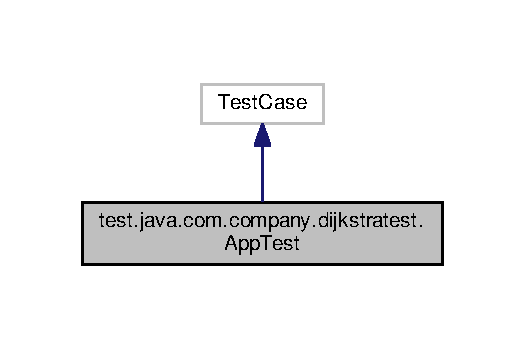
\includegraphics[width=252pt]{classtest_1_1java_1_1com_1_1company_1_1dijkstratest_1_1_app_test__inherit__graph}
\end{center}
\end{figure}


Collaboration diagram for test.\-java.\-com.\-company.\-dijkstratest.\-App\-Test\-:
\nopagebreak
\begin{figure}[H]
\begin{center}
\leavevmode
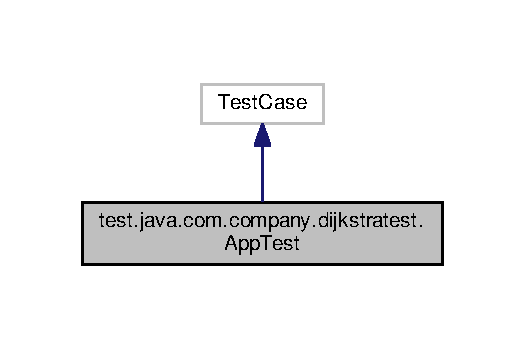
\includegraphics[width=252pt]{classtest_1_1java_1_1com_1_1company_1_1dijkstratest_1_1_app_test__coll__graph}
\end{center}
\end{figure}
\subsection*{Public Member Functions}
\begin{DoxyCompactItemize}
\item 
\hyperlink{classtest_1_1java_1_1com_1_1company_1_1dijkstratest_1_1_app_test_ab8981b2f8304e8c357c461c6fcc4a0ef}{App\-Test} (String test\-Name)
\item 
void \hyperlink{classtest_1_1java_1_1com_1_1company_1_1dijkstratest_1_1_app_test_a8a8c57d59a43320f7dcc1e03ecf6050c}{test\-App} ()
\end{DoxyCompactItemize}
\subsection*{Static Public Member Functions}
\begin{DoxyCompactItemize}
\item 
static Test \hyperlink{classtest_1_1java_1_1com_1_1company_1_1dijkstratest_1_1_app_test_af663b7af9263e3cf82aedb00b10ef0ca}{suite} ()
\end{DoxyCompactItemize}


\subsection{Detailed Description}
Unit test for simple App. 

Definition at line 10 of file App\-Test.\-java.



\subsection{Constructor \& Destructor Documentation}
\hypertarget{classtest_1_1java_1_1com_1_1company_1_1dijkstratest_1_1_app_test_ab8981b2f8304e8c357c461c6fcc4a0ef}{\index{test\-::java\-::com\-::company\-::dijkstratest\-::\-App\-Test@{test\-::java\-::com\-::company\-::dijkstratest\-::\-App\-Test}!App\-Test@{App\-Test}}
\index{App\-Test@{App\-Test}!test::java::com::company::dijkstratest::AppTest@{test\-::java\-::com\-::company\-::dijkstratest\-::\-App\-Test}}
\subsubsection[{App\-Test}]{\setlength{\rightskip}{0pt plus 5cm}test.\-java.\-com.\-company.\-dijkstratest.\-App\-Test.\-App\-Test (
\begin{DoxyParamCaption}
\item[{String}]{test\-Name}
\end{DoxyParamCaption}
)}}\label{classtest_1_1java_1_1com_1_1company_1_1dijkstratest_1_1_app_test_ab8981b2f8304e8c357c461c6fcc4a0ef}
Create the test case


\begin{DoxyParams}{Parameters}
{\em test\-Name} & name of the test case \\
\hline
\end{DoxyParams}


Definition at line 18 of file App\-Test.\-java.



\subsection{Member Function Documentation}
\hypertarget{classtest_1_1java_1_1com_1_1company_1_1dijkstratest_1_1_app_test_af663b7af9263e3cf82aedb00b10ef0ca}{\index{test\-::java\-::com\-::company\-::dijkstratest\-::\-App\-Test@{test\-::java\-::com\-::company\-::dijkstratest\-::\-App\-Test}!suite@{suite}}
\index{suite@{suite}!test::java::com::company::dijkstratest::AppTest@{test\-::java\-::com\-::company\-::dijkstratest\-::\-App\-Test}}
\subsubsection[{suite}]{\setlength{\rightskip}{0pt plus 5cm}static Test test.\-java.\-com.\-company.\-dijkstratest.\-App\-Test.\-suite (
\begin{DoxyParamCaption}
{}
\end{DoxyParamCaption}
)\hspace{0.3cm}{\ttfamily [static]}}}\label{classtest_1_1java_1_1com_1_1company_1_1dijkstratest_1_1_app_test_af663b7af9263e3cf82aedb00b10ef0ca}
\begin{DoxyReturn}{Returns}
the suite of tests being tested 
\end{DoxyReturn}


Definition at line 26 of file App\-Test.\-java.

\hypertarget{classtest_1_1java_1_1com_1_1company_1_1dijkstratest_1_1_app_test_a8a8c57d59a43320f7dcc1e03ecf6050c}{\index{test\-::java\-::com\-::company\-::dijkstratest\-::\-App\-Test@{test\-::java\-::com\-::company\-::dijkstratest\-::\-App\-Test}!test\-App@{test\-App}}
\index{test\-App@{test\-App}!test::java::com::company::dijkstratest::AppTest@{test\-::java\-::com\-::company\-::dijkstratest\-::\-App\-Test}}
\subsubsection[{test\-App}]{\setlength{\rightskip}{0pt plus 5cm}void test.\-java.\-com.\-company.\-dijkstratest.\-App\-Test.\-test\-App (
\begin{DoxyParamCaption}
{}
\end{DoxyParamCaption}
)}}\label{classtest_1_1java_1_1com_1_1company_1_1dijkstratest_1_1_app_test_a8a8c57d59a43320f7dcc1e03ecf6050c}
Rigourous Test \-:-\/) 

Definition at line 34 of file App\-Test.\-java.



The documentation for this class was generated from the following file\-:\begin{DoxyCompactItemize}
\item 
src/test/java/com/company/dijkstratest/\hyperlink{_app_test_8java}{App\-Test.\-java}\end{DoxyCompactItemize}

\hypertarget{classmain_1_1java_1_1com_1_1company_1_1dijkstratest_1_1_community}{\section{main.\-java.\-com.\-company.\-dijkstratest.\-Community Class Reference}
\label{classmain_1_1java_1_1com_1_1company_1_1dijkstratest_1_1_community}\index{main.\-java.\-com.\-company.\-dijkstratest.\-Community@{main.\-java.\-com.\-company.\-dijkstratest.\-Community}}
}


Collaboration diagram for main.\-java.\-com.\-company.\-dijkstratest.\-Community\-:
\nopagebreak
\begin{figure}[H]
\begin{center}
\leavevmode
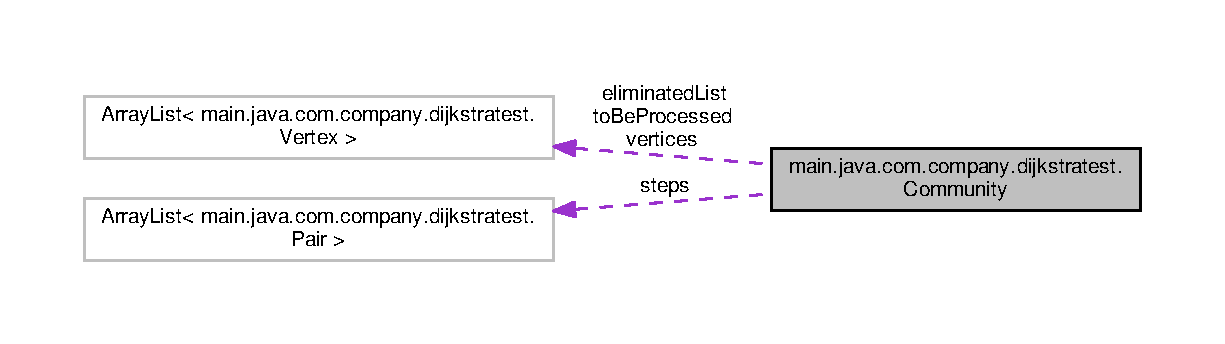
\includegraphics[width=350pt]{classmain_1_1java_1_1com_1_1company_1_1dijkstratest_1_1_community__coll__graph}
\end{center}
\end{figure}
\subsection*{Public Member Functions}
\begin{DoxyCompactItemize}
\item 
\hyperlink{classmain_1_1java_1_1com_1_1company_1_1dijkstratest_1_1_community_a948a27b50995af847cd53c449349ed7c}{Community} (Array\-List$<$ \hyperlink{classmain_1_1java_1_1com_1_1company_1_1dijkstratest_1_1_vertex}{Vertex} $>$ \hyperlink{classmain_1_1java_1_1com_1_1company_1_1dijkstratest_1_1_community_a00e314391bafea784ad183152dcd6091}{vertices}, Array\-List$<$ \hyperlink{classmain_1_1java_1_1com_1_1company_1_1dijkstratest_1_1_vertex}{Vertex} $>$ \hyperlink{classmain_1_1java_1_1com_1_1company_1_1dijkstratest_1_1_community_a2ccabf2789253dffe72aa412e7412f7d}{to\-Be\-Processed}, Array\-List$<$ \hyperlink{classmain_1_1java_1_1com_1_1company_1_1dijkstratest_1_1_vertex}{Vertex} $>$ \hyperlink{classmain_1_1java_1_1com_1_1company_1_1dijkstratest_1_1_community_a580104f4f16e9646bb1c4b3ea36c20a5}{eliminated\-List})
\item 
Array\-List$<$ \hyperlink{classmain_1_1java_1_1com_1_1company_1_1dijkstratest_1_1_vertex}{Vertex} $>$ \hyperlink{classmain_1_1java_1_1com_1_1company_1_1dijkstratest_1_1_community_ac67908826386b0b27d640714ddca078c}{build\-Community} ()
\item 
\hyperlink{classmain_1_1java_1_1com_1_1company_1_1dijkstratest_1_1_vertex}{Vertex} \hyperlink{classmain_1_1java_1_1com_1_1company_1_1dijkstratest_1_1_community_af8ba9d3ca770ca1683efe6e0b842d2d5}{get\-Highest\-Centralitied} ()
\item 
Array\-List$<$ \hyperlink{classmain_1_1java_1_1com_1_1company_1_1dijkstratest_1_1_vertex}{Vertex} $>$ \hyperlink{classmain_1_1java_1_1com_1_1company_1_1dijkstratest_1_1_community_a11c0953e985a94460b905218c3c80291}{get\-Community\-Candidates} (\hyperlink{classmain_1_1java_1_1com_1_1company_1_1dijkstratest_1_1_vertex}{Vertex} highest)
\item 
void \hyperlink{classmain_1_1java_1_1com_1_1company_1_1dijkstratest_1_1_community_aba4c016c6178f4b4f6e2a29874c0c619}{delete\-Candidates} (Array\-List$<$ \hyperlink{classmain_1_1java_1_1com_1_1company_1_1dijkstratest_1_1_vertex}{Vertex} $>$ c\-Candidates)
\item 
boolean \hyperlink{classmain_1_1java_1_1com_1_1company_1_1dijkstratest_1_1_community_ab4d06c5bd90490a5713b1aa083cdeef9}{is\-Isolated} (\hyperlink{classmain_1_1java_1_1com_1_1company_1_1dijkstratest_1_1_vertex}{Vertex} v)
\end{DoxyCompactItemize}
\subsection*{Private Member Functions}
\begin{DoxyCompactItemize}
\item 
void \hyperlink{classmain_1_1java_1_1com_1_1company_1_1dijkstratest_1_1_community_aba69300314e63161ff7e0a3b5aebe2ad}{reset\-Steps} ()
\end{DoxyCompactItemize}
\subsection*{Private Attributes}
\begin{DoxyCompactItemize}
\item 
Array\-List$<$ \hyperlink{classmain_1_1java_1_1com_1_1company_1_1dijkstratest_1_1_vertex}{Vertex} $>$ \hyperlink{classmain_1_1java_1_1com_1_1company_1_1dijkstratest_1_1_community_a00e314391bafea784ad183152dcd6091}{vertices}
\item 
Array\-List$<$ \hyperlink{classmain_1_1java_1_1com_1_1company_1_1dijkstratest_1_1_vertex}{Vertex} $>$ \hyperlink{classmain_1_1java_1_1com_1_1company_1_1dijkstratest_1_1_community_a2ccabf2789253dffe72aa412e7412f7d}{to\-Be\-Processed}
\item 
Array\-List$<$ \hyperlink{classmain_1_1java_1_1com_1_1company_1_1dijkstratest_1_1_vertex}{Vertex} $>$ \hyperlink{classmain_1_1java_1_1com_1_1company_1_1dijkstratest_1_1_community_a580104f4f16e9646bb1c4b3ea36c20a5}{eliminated\-List}
\item 
Array\-List$<$ \hyperlink{classmain_1_1java_1_1com_1_1company_1_1dijkstratest_1_1_pair}{Pair} $>$ \hyperlink{classmain_1_1java_1_1com_1_1company_1_1dijkstratest_1_1_community_adbb6dc448c6e9ffdcd3207b5117e5ac6}{steps}
\end{DoxyCompactItemize}


\subsection{Detailed Description}
\hyperlink{classmain_1_1java_1_1com_1_1company_1_1dijkstratest_1_1_community}{Community} is to find all the community candidates \begin{DoxyAuthor}{Author}
hzhang 
\end{DoxyAuthor}


Definition at line 10 of file Community.\-java.



\subsection{Constructor \& Destructor Documentation}
\hypertarget{classmain_1_1java_1_1com_1_1company_1_1dijkstratest_1_1_community_a948a27b50995af847cd53c449349ed7c}{\index{main\-::java\-::com\-::company\-::dijkstratest\-::\-Community@{main\-::java\-::com\-::company\-::dijkstratest\-::\-Community}!Community@{Community}}
\index{Community@{Community}!main::java::com::company::dijkstratest::Community@{main\-::java\-::com\-::company\-::dijkstratest\-::\-Community}}
\subsubsection[{Community}]{\setlength{\rightskip}{0pt plus 5cm}main.\-java.\-com.\-company.\-dijkstratest.\-Community.\-Community (
\begin{DoxyParamCaption}
\item[{Array\-List$<$ {\bf Vertex} $>$}]{vertices, }
\item[{Array\-List$<$ {\bf Vertex} $>$}]{to\-Be\-Processed, }
\item[{Array\-List$<$ {\bf Vertex} $>$}]{eliminated\-List}
\end{DoxyParamCaption}
)}}\label{classmain_1_1java_1_1com_1_1company_1_1dijkstratest_1_1_community_a948a27b50995af847cd53c449349ed7c}


Definition at line 17 of file Community.\-java.



References main.\-java.\-com.\-company.\-dijkstratest.\-Community.\-eliminated\-List, main.\-java.\-com.\-company.\-dijkstratest.\-Community.\-reset\-Steps(), main.\-java.\-com.\-company.\-dijkstratest.\-Community.\-to\-Be\-Processed, and main.\-java.\-com.\-company.\-dijkstratest.\-Community.\-vertices.



Here is the call graph for this function\-:
\nopagebreak
\begin{figure}[H]
\begin{center}
\leavevmode
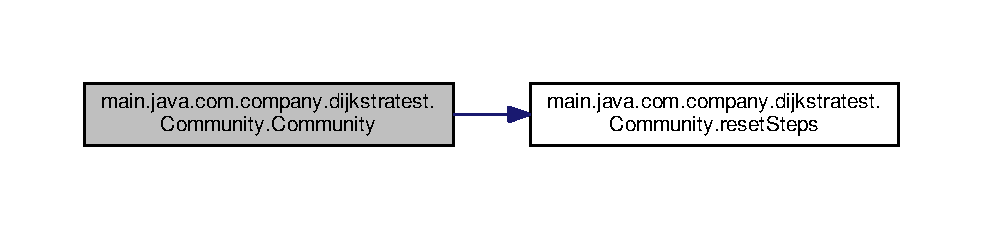
\includegraphics[width=350pt]{classmain_1_1java_1_1com_1_1company_1_1dijkstratest_1_1_community_a948a27b50995af847cd53c449349ed7c_cgraph}
\end{center}
\end{figure}




\subsection{Member Function Documentation}
\hypertarget{classmain_1_1java_1_1com_1_1company_1_1dijkstratest_1_1_community_ac67908826386b0b27d640714ddca078c}{\index{main\-::java\-::com\-::company\-::dijkstratest\-::\-Community@{main\-::java\-::com\-::company\-::dijkstratest\-::\-Community}!build\-Community@{build\-Community}}
\index{build\-Community@{build\-Community}!main::java::com::company::dijkstratest::Community@{main\-::java\-::com\-::company\-::dijkstratest\-::\-Community}}
\subsubsection[{build\-Community}]{\setlength{\rightskip}{0pt plus 5cm}Array\-List$<${\bf Vertex}$>$ main.\-java.\-com.\-company.\-dijkstratest.\-Community.\-build\-Community (
\begin{DoxyParamCaption}
{}
\end{DoxyParamCaption}
)}}\label{classmain_1_1java_1_1com_1_1company_1_1dijkstratest_1_1_community_ac67908826386b0b27d640714ddca078c}
Build \hyperlink{classmain_1_1java_1_1com_1_1company_1_1dijkstratest_1_1_community}{Community} 

Definition at line 29 of file Community.\-java.



References main.\-java.\-com.\-company.\-dijkstratest.\-Community.\-delete\-Candidates(), main.\-java.\-com.\-company.\-dijkstratest.\-Community.\-get\-Community\-Candidates(), main.\-java.\-com.\-company.\-dijkstratest.\-Community.\-get\-Highest\-Centralitied(), and main.\-java.\-com.\-company.\-dijkstratest.\-Community.\-to\-Be\-Processed.



Here is the call graph for this function\-:
\nopagebreak
\begin{figure}[H]
\begin{center}
\leavevmode
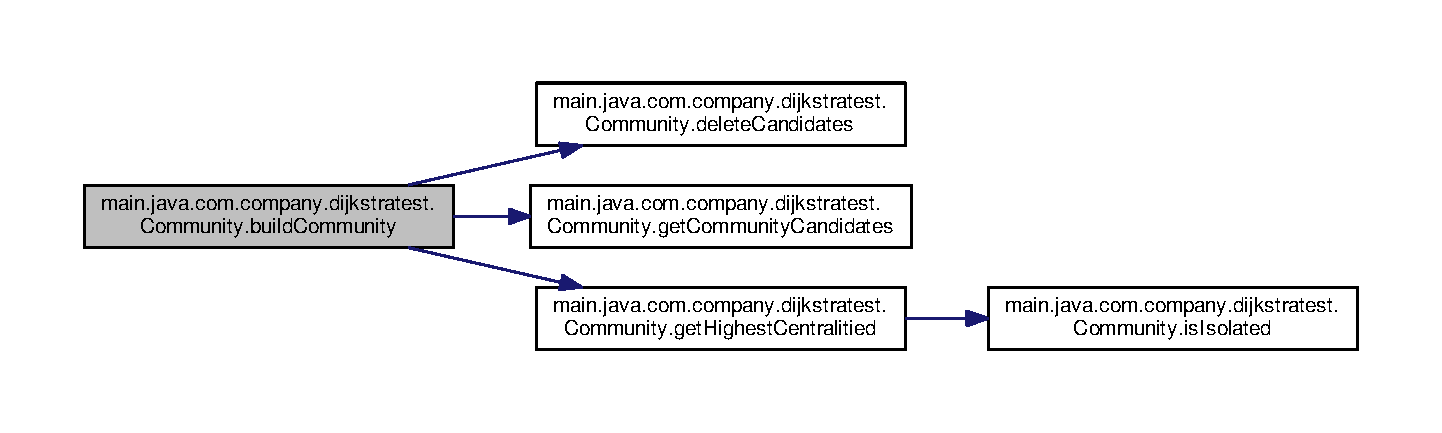
\includegraphics[width=350pt]{classmain_1_1java_1_1com_1_1company_1_1dijkstratest_1_1_community_ac67908826386b0b27d640714ddca078c_cgraph}
\end{center}
\end{figure}


\hypertarget{classmain_1_1java_1_1com_1_1company_1_1dijkstratest_1_1_community_aba4c016c6178f4b4f6e2a29874c0c619}{\index{main\-::java\-::com\-::company\-::dijkstratest\-::\-Community@{main\-::java\-::com\-::company\-::dijkstratest\-::\-Community}!delete\-Candidates@{delete\-Candidates}}
\index{delete\-Candidates@{delete\-Candidates}!main::java::com::company::dijkstratest::Community@{main\-::java\-::com\-::company\-::dijkstratest\-::\-Community}}
\subsubsection[{delete\-Candidates}]{\setlength{\rightskip}{0pt plus 5cm}void main.\-java.\-com.\-company.\-dijkstratest.\-Community.\-delete\-Candidates (
\begin{DoxyParamCaption}
\item[{Array\-List$<$ {\bf Vertex} $>$}]{c\-Candidates}
\end{DoxyParamCaption}
)}}\label{classmain_1_1java_1_1com_1_1company_1_1dijkstratest_1_1_community_aba4c016c6178f4b4f6e2a29874c0c619}
Delete community candidates from the original vertices 
\begin{DoxyParams}{Parameters}
{\em c\-Candidates} & \\
\hline
\end{DoxyParams}


Definition at line 84 of file Community.\-java.



Referenced by main.\-java.\-com.\-company.\-dijkstratest.\-Community.\-build\-Community().

\hypertarget{classmain_1_1java_1_1com_1_1company_1_1dijkstratest_1_1_community_a11c0953e985a94460b905218c3c80291}{\index{main\-::java\-::com\-::company\-::dijkstratest\-::\-Community@{main\-::java\-::com\-::company\-::dijkstratest\-::\-Community}!get\-Community\-Candidates@{get\-Community\-Candidates}}
\index{get\-Community\-Candidates@{get\-Community\-Candidates}!main::java::com::company::dijkstratest::Community@{main\-::java\-::com\-::company\-::dijkstratest\-::\-Community}}
\subsubsection[{get\-Community\-Candidates}]{\setlength{\rightskip}{0pt plus 5cm}Array\-List$<${\bf Vertex}$>$ main.\-java.\-com.\-company.\-dijkstratest.\-Community.\-get\-Community\-Candidates (
\begin{DoxyParamCaption}
\item[{{\bf Vertex}}]{highest}
\end{DoxyParamCaption}
)}}\label{classmain_1_1java_1_1com_1_1company_1_1dijkstratest_1_1_community_a11c0953e985a94460b905218c3c80291}
Get the vertices which belong to the community


\begin{DoxyParams}{Parameters}
{\em highest} & \\
\hline
\end{DoxyParams}
\begin{DoxyReturn}{Returns}

\end{DoxyReturn}


Definition at line 65 of file Community.\-java.



References main.\-java.\-com.\-company.\-dijkstratest.\-Community.\-steps.



Referenced by main.\-java.\-com.\-company.\-dijkstratest.\-Community.\-build\-Community().

\hypertarget{classmain_1_1java_1_1com_1_1company_1_1dijkstratest_1_1_community_af8ba9d3ca770ca1683efe6e0b842d2d5}{\index{main\-::java\-::com\-::company\-::dijkstratest\-::\-Community@{main\-::java\-::com\-::company\-::dijkstratest\-::\-Community}!get\-Highest\-Centralitied@{get\-Highest\-Centralitied}}
\index{get\-Highest\-Centralitied@{get\-Highest\-Centralitied}!main::java::com::company::dijkstratest::Community@{main\-::java\-::com\-::company\-::dijkstratest\-::\-Community}}
\subsubsection[{get\-Highest\-Centralitied}]{\setlength{\rightskip}{0pt plus 5cm}{\bf Vertex} main.\-java.\-com.\-company.\-dijkstratest.\-Community.\-get\-Highest\-Centralitied (
\begin{DoxyParamCaption}
{}
\end{DoxyParamCaption}
)}}\label{classmain_1_1java_1_1com_1_1company_1_1dijkstratest_1_1_community_af8ba9d3ca770ca1683efe6e0b842d2d5}
Get the vertex which has the highest centrality/smallest diameter

\begin{DoxyReturn}{Returns}
highest vertex 
\end{DoxyReturn}


Definition at line 43 of file Community.\-java.



References main.\-java.\-com.\-company.\-dijkstratest.\-Community.\-is\-Isolated(), and main.\-java.\-com.\-company.\-dijkstratest.\-Community.\-vertices.



Referenced by main.\-java.\-com.\-company.\-dijkstratest.\-Community.\-build\-Community().



Here is the call graph for this function\-:
\nopagebreak
\begin{figure}[H]
\begin{center}
\leavevmode
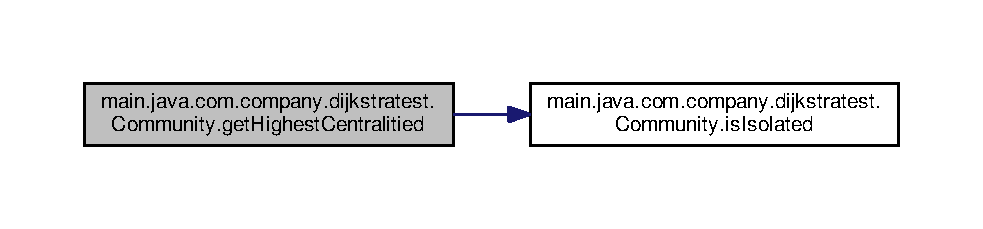
\includegraphics[width=350pt]{classmain_1_1java_1_1com_1_1company_1_1dijkstratest_1_1_community_af8ba9d3ca770ca1683efe6e0b842d2d5_cgraph}
\end{center}
\end{figure}


\hypertarget{classmain_1_1java_1_1com_1_1company_1_1dijkstratest_1_1_community_ab4d06c5bd90490a5713b1aa083cdeef9}{\index{main\-::java\-::com\-::company\-::dijkstratest\-::\-Community@{main\-::java\-::com\-::company\-::dijkstratest\-::\-Community}!is\-Isolated@{is\-Isolated}}
\index{is\-Isolated@{is\-Isolated}!main::java::com::company::dijkstratest::Community@{main\-::java\-::com\-::company\-::dijkstratest\-::\-Community}}
\subsubsection[{is\-Isolated}]{\setlength{\rightskip}{0pt plus 5cm}boolean main.\-java.\-com.\-company.\-dijkstratest.\-Community.\-is\-Isolated (
\begin{DoxyParamCaption}
\item[{{\bf Vertex}}]{v}
\end{DoxyParamCaption}
)}}\label{classmain_1_1java_1_1com_1_1company_1_1dijkstratest_1_1_community_ab4d06c5bd90490a5713b1aa083cdeef9}
Checking whether a vertex is isolated If it is, it will not be chosen as a highest centrality vertex. 
\begin{DoxyParams}{Parameters}
{\em v} & \\
\hline
\end{DoxyParams}
\begin{DoxyReturn}{Returns}

\end{DoxyReturn}


Definition at line 101 of file Community.\-java.



Referenced by main.\-java.\-com.\-company.\-dijkstratest.\-Community.\-get\-Highest\-Centralitied().

\hypertarget{classmain_1_1java_1_1com_1_1company_1_1dijkstratest_1_1_community_aba69300314e63161ff7e0a3b5aebe2ad}{\index{main\-::java\-::com\-::company\-::dijkstratest\-::\-Community@{main\-::java\-::com\-::company\-::dijkstratest\-::\-Community}!reset\-Steps@{reset\-Steps}}
\index{reset\-Steps@{reset\-Steps}!main::java::com::company::dijkstratest::Community@{main\-::java\-::com\-::company\-::dijkstratest\-::\-Community}}
\subsubsection[{reset\-Steps}]{\setlength{\rightskip}{0pt plus 5cm}void main.\-java.\-com.\-company.\-dijkstratest.\-Community.\-reset\-Steps (
\begin{DoxyParamCaption}
{}
\end{DoxyParamCaption}
)\hspace{0.3cm}{\ttfamily [private]}}}\label{classmain_1_1java_1_1com_1_1company_1_1dijkstratest_1_1_community_aba69300314e63161ff7e0a3b5aebe2ad}
Set the steps to the eliminated vertex to be I\-N\-F\-I\-N\-I\-T\-Y. 

Definition at line 123 of file Community.\-java.



References main.\-java.\-com.\-company.\-dijkstratest.\-Community.\-eliminated\-List, and main.\-java.\-com.\-company.\-dijkstratest.\-Community.\-vertices.



Referenced by main.\-java.\-com.\-company.\-dijkstratest.\-Community.\-Community().



\subsection{Member Data Documentation}
\hypertarget{classmain_1_1java_1_1com_1_1company_1_1dijkstratest_1_1_community_a580104f4f16e9646bb1c4b3ea36c20a5}{\index{main\-::java\-::com\-::company\-::dijkstratest\-::\-Community@{main\-::java\-::com\-::company\-::dijkstratest\-::\-Community}!eliminated\-List@{eliminated\-List}}
\index{eliminated\-List@{eliminated\-List}!main::java::com::company::dijkstratest::Community@{main\-::java\-::com\-::company\-::dijkstratest\-::\-Community}}
\subsubsection[{eliminated\-List}]{\setlength{\rightskip}{0pt plus 5cm}Array\-List$<${\bf Vertex}$>$ main.\-java.\-com.\-company.\-dijkstratest.\-Community.\-eliminated\-List\hspace{0.3cm}{\ttfamily [private]}}}\label{classmain_1_1java_1_1com_1_1company_1_1dijkstratest_1_1_community_a580104f4f16e9646bb1c4b3ea36c20a5}


Definition at line 14 of file Community.\-java.



Referenced by main.\-java.\-com.\-company.\-dijkstratest.\-Community.\-Community(), and main.\-java.\-com.\-company.\-dijkstratest.\-Community.\-reset\-Steps().

\hypertarget{classmain_1_1java_1_1com_1_1company_1_1dijkstratest_1_1_community_adbb6dc448c6e9ffdcd3207b5117e5ac6}{\index{main\-::java\-::com\-::company\-::dijkstratest\-::\-Community@{main\-::java\-::com\-::company\-::dijkstratest\-::\-Community}!steps@{steps}}
\index{steps@{steps}!main::java::com::company::dijkstratest::Community@{main\-::java\-::com\-::company\-::dijkstratest\-::\-Community}}
\subsubsection[{steps}]{\setlength{\rightskip}{0pt plus 5cm}Array\-List$<${\bf Pair}$>$ main.\-java.\-com.\-company.\-dijkstratest.\-Community.\-steps\hspace{0.3cm}{\ttfamily [private]}}}\label{classmain_1_1java_1_1com_1_1company_1_1dijkstratest_1_1_community_adbb6dc448c6e9ffdcd3207b5117e5ac6}


Definition at line 15 of file Community.\-java.



Referenced by main.\-java.\-com.\-company.\-dijkstratest.\-Community.\-get\-Community\-Candidates().

\hypertarget{classmain_1_1java_1_1com_1_1company_1_1dijkstratest_1_1_community_a2ccabf2789253dffe72aa412e7412f7d}{\index{main\-::java\-::com\-::company\-::dijkstratest\-::\-Community@{main\-::java\-::com\-::company\-::dijkstratest\-::\-Community}!to\-Be\-Processed@{to\-Be\-Processed}}
\index{to\-Be\-Processed@{to\-Be\-Processed}!main::java::com::company::dijkstratest::Community@{main\-::java\-::com\-::company\-::dijkstratest\-::\-Community}}
\subsubsection[{to\-Be\-Processed}]{\setlength{\rightskip}{0pt plus 5cm}Array\-List$<${\bf Vertex}$>$ main.\-java.\-com.\-company.\-dijkstratest.\-Community.\-to\-Be\-Processed\hspace{0.3cm}{\ttfamily [private]}}}\label{classmain_1_1java_1_1com_1_1company_1_1dijkstratest_1_1_community_a2ccabf2789253dffe72aa412e7412f7d}


Definition at line 13 of file Community.\-java.



Referenced by main.\-java.\-com.\-company.\-dijkstratest.\-Community.\-build\-Community(), and main.\-java.\-com.\-company.\-dijkstratest.\-Community.\-Community().

\hypertarget{classmain_1_1java_1_1com_1_1company_1_1dijkstratest_1_1_community_a00e314391bafea784ad183152dcd6091}{\index{main\-::java\-::com\-::company\-::dijkstratest\-::\-Community@{main\-::java\-::com\-::company\-::dijkstratest\-::\-Community}!vertices@{vertices}}
\index{vertices@{vertices}!main::java::com::company::dijkstratest::Community@{main\-::java\-::com\-::company\-::dijkstratest\-::\-Community}}
\subsubsection[{vertices}]{\setlength{\rightskip}{0pt plus 5cm}Array\-List$<${\bf Vertex}$>$ main.\-java.\-com.\-company.\-dijkstratest.\-Community.\-vertices\hspace{0.3cm}{\ttfamily [private]}}}\label{classmain_1_1java_1_1com_1_1company_1_1dijkstratest_1_1_community_a00e314391bafea784ad183152dcd6091}


Definition at line 12 of file Community.\-java.



Referenced by main.\-java.\-com.\-company.\-dijkstratest.\-Community.\-Community(), main.\-java.\-com.\-company.\-dijkstratest.\-Community.\-get\-Highest\-Centralitied(), and main.\-java.\-com.\-company.\-dijkstratest.\-Community.\-reset\-Steps().



The documentation for this class was generated from the following file\-:\begin{DoxyCompactItemize}
\item 
src/main/java/com/company/dijkstratest/\hyperlink{_community_8java}{Community.\-java}\end{DoxyCompactItemize}

\hypertarget{classmain_1_1java_1_1com_1_1company_1_1dijkstratest_1_1_connection_matrix}{\section{main.\-java.\-com.\-company.\-dijkstratest.\-Connection\-Matrix Class Reference}
\label{classmain_1_1java_1_1com_1_1company_1_1dijkstratest_1_1_connection_matrix}\index{main.\-java.\-com.\-company.\-dijkstratest.\-Connection\-Matrix@{main.\-java.\-com.\-company.\-dijkstratest.\-Connection\-Matrix}}
}


Collaboration diagram for main.\-java.\-com.\-company.\-dijkstratest.\-Connection\-Matrix\-:
\nopagebreak
\begin{figure}[H]
\begin{center}
\leavevmode
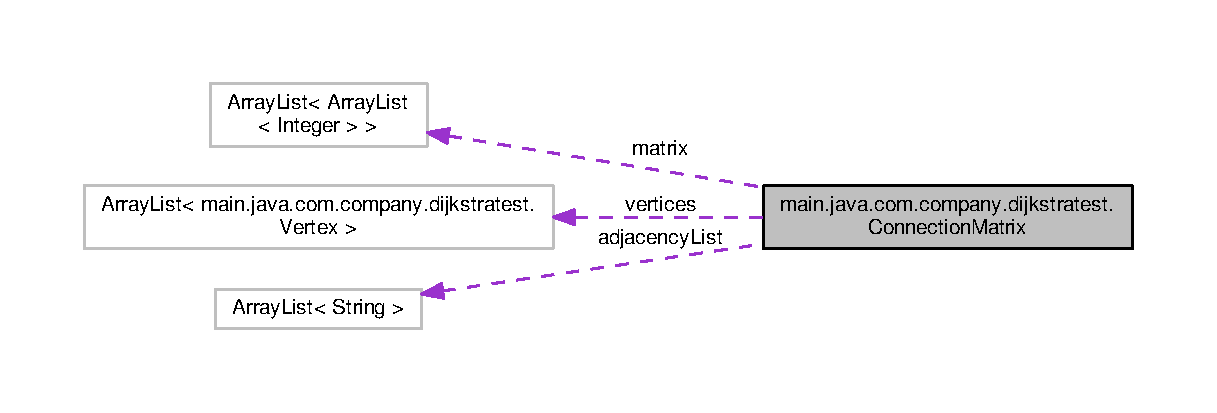
\includegraphics[width=350pt]{classmain_1_1java_1_1com_1_1company_1_1dijkstratest_1_1_connection_matrix__coll__graph}
\end{center}
\end{figure}
\subsection*{Public Member Functions}
\begin{DoxyCompactItemize}
\item 
\hyperlink{classmain_1_1java_1_1com_1_1company_1_1dijkstratest_1_1_connection_matrix_abf29234358773911d627a62f49502e95}{Connection\-Matrix} (Array\-List$<$ \hyperlink{classmain_1_1java_1_1com_1_1company_1_1dijkstratest_1_1_vertex}{Vertex} $>$ \hyperlink{classmain_1_1java_1_1com_1_1company_1_1dijkstratest_1_1_connection_matrix_a372aa9baecc703f490a3eef8845bc7a7}{vertices}, Array\-List$<$ String $>$ \hyperlink{classmain_1_1java_1_1com_1_1company_1_1dijkstratest_1_1_connection_matrix_a0fcd8b3828105bd570fd97dca77db1ea}{adjacency\-List})
\item 
void \hyperlink{classmain_1_1java_1_1com_1_1company_1_1dijkstratest_1_1_connection_matrix_a883880082124638cae78f50746006e5b}{build\-Connection\-Matrix} ()
\item 
void \hyperlink{classmain_1_1java_1_1com_1_1company_1_1dijkstratest_1_1_connection_matrix_ade4179ca5619dadb5a2bbadab52ac93e}{register\-Adjacencies\-To\-Each\-Vertex} ()
\item 
String\mbox{[}$\,$\mbox{]} \hyperlink{classmain_1_1java_1_1com_1_1company_1_1dijkstratest_1_1_connection_matrix_a40c35866fd543064f675971e91a88a75}{split\-Op\-Cp} (String op\-Cp)
\item 
void \hyperlink{classmain_1_1java_1_1com_1_1company_1_1dijkstratest_1_1_connection_matrix_ab761efa04c328a3362d653a6612dd404}{fill\-Grid} ()
\item 
void \hyperlink{classmain_1_1java_1_1com_1_1company_1_1dijkstratest_1_1_connection_matrix_ad305dcd4ab25d7628dd843451e1856be}{display\-Connection\-Matrix} ()
\end{DoxyCompactItemize}
\subsection*{Private Attributes}
\begin{DoxyCompactItemize}
\item 
final Array\-List$<$ String $>$ \hyperlink{classmain_1_1java_1_1com_1_1company_1_1dijkstratest_1_1_connection_matrix_a0fcd8b3828105bd570fd97dca77db1ea}{adjacency\-List}
\item 
final Array\-List$<$ \hyperlink{classmain_1_1java_1_1com_1_1company_1_1dijkstratest_1_1_vertex}{Vertex} $>$ \hyperlink{classmain_1_1java_1_1com_1_1company_1_1dijkstratest_1_1_connection_matrix_a372aa9baecc703f490a3eef8845bc7a7}{vertices}
\item 
final Array\-List$<$ Array\-List\\*
$<$ Integer $>$ $>$ \hyperlink{classmain_1_1java_1_1com_1_1company_1_1dijkstratest_1_1_connection_matrix_a3c077791f0b8164d8c19f67d250f43fd}{matrix} = new Array\-List$<$Array\-List$<$Integer$>$$>$()
\end{DoxyCompactItemize}


\subsection{Detailed Description}
Find the neighbor-\/relationship among all subscribers, and then build a connection matrix based on the neighborhood relationship

\begin{DoxyAuthor}{Author}
hzhang 
\end{DoxyAuthor}


Definition at line 11 of file Connection\-Matrix.\-java.



\subsection{Constructor \& Destructor Documentation}
\hypertarget{classmain_1_1java_1_1com_1_1company_1_1dijkstratest_1_1_connection_matrix_abf29234358773911d627a62f49502e95}{\index{main\-::java\-::com\-::company\-::dijkstratest\-::\-Connection\-Matrix@{main\-::java\-::com\-::company\-::dijkstratest\-::\-Connection\-Matrix}!Connection\-Matrix@{Connection\-Matrix}}
\index{Connection\-Matrix@{Connection\-Matrix}!main::java::com::company::dijkstratest::ConnectionMatrix@{main\-::java\-::com\-::company\-::dijkstratest\-::\-Connection\-Matrix}}
\subsubsection[{Connection\-Matrix}]{\setlength{\rightskip}{0pt plus 5cm}main.\-java.\-com.\-company.\-dijkstratest.\-Connection\-Matrix.\-Connection\-Matrix (
\begin{DoxyParamCaption}
\item[{Array\-List$<$ {\bf Vertex} $>$}]{vertices, }
\item[{Array\-List$<$ String $>$}]{adjacency\-List}
\end{DoxyParamCaption}
)}}\label{classmain_1_1java_1_1com_1_1company_1_1dijkstratest_1_1_connection_matrix_abf29234358773911d627a62f49502e95}
Constructor


\begin{DoxyParams}{Parameters}
{\em subscribers\-List} & list of all subscribers \\
\hline
{\em adjacency\-List} & list of all neighbors \\
\hline
\end{DoxyParams}


Definition at line 23 of file Connection\-Matrix.\-java.



References main.\-java.\-com.\-company.\-dijkstratest.\-Connection\-Matrix.\-adjacency\-List, and main.\-java.\-com.\-company.\-dijkstratest.\-Connection\-Matrix.\-vertices.



\subsection{Member Function Documentation}
\hypertarget{classmain_1_1java_1_1com_1_1company_1_1dijkstratest_1_1_connection_matrix_a883880082124638cae78f50746006e5b}{\index{main\-::java\-::com\-::company\-::dijkstratest\-::\-Connection\-Matrix@{main\-::java\-::com\-::company\-::dijkstratest\-::\-Connection\-Matrix}!build\-Connection\-Matrix@{build\-Connection\-Matrix}}
\index{build\-Connection\-Matrix@{build\-Connection\-Matrix}!main::java::com::company::dijkstratest::ConnectionMatrix@{main\-::java\-::com\-::company\-::dijkstratest\-::\-Connection\-Matrix}}
\subsubsection[{build\-Connection\-Matrix}]{\setlength{\rightskip}{0pt plus 5cm}void main.\-java.\-com.\-company.\-dijkstratest.\-Connection\-Matrix.\-build\-Connection\-Matrix (
\begin{DoxyParamCaption}
{}
\end{DoxyParamCaption}
)}}\label{classmain_1_1java_1_1com_1_1company_1_1dijkstratest_1_1_connection_matrix_a883880082124638cae78f50746006e5b}


Definition at line 29 of file Connection\-Matrix.\-java.



References main.\-java.\-com.\-company.\-dijkstratest.\-Connection\-Matrix.\-display\-Connection\-Matrix(), main.\-java.\-com.\-company.\-dijkstratest.\-Connection\-Matrix.\-fill\-Grid(), and main.\-java.\-com.\-company.\-dijkstratest.\-Connection\-Matrix.\-register\-Adjacencies\-To\-Each\-Vertex().



Here is the call graph for this function\-:
\nopagebreak
\begin{figure}[H]
\begin{center}
\leavevmode
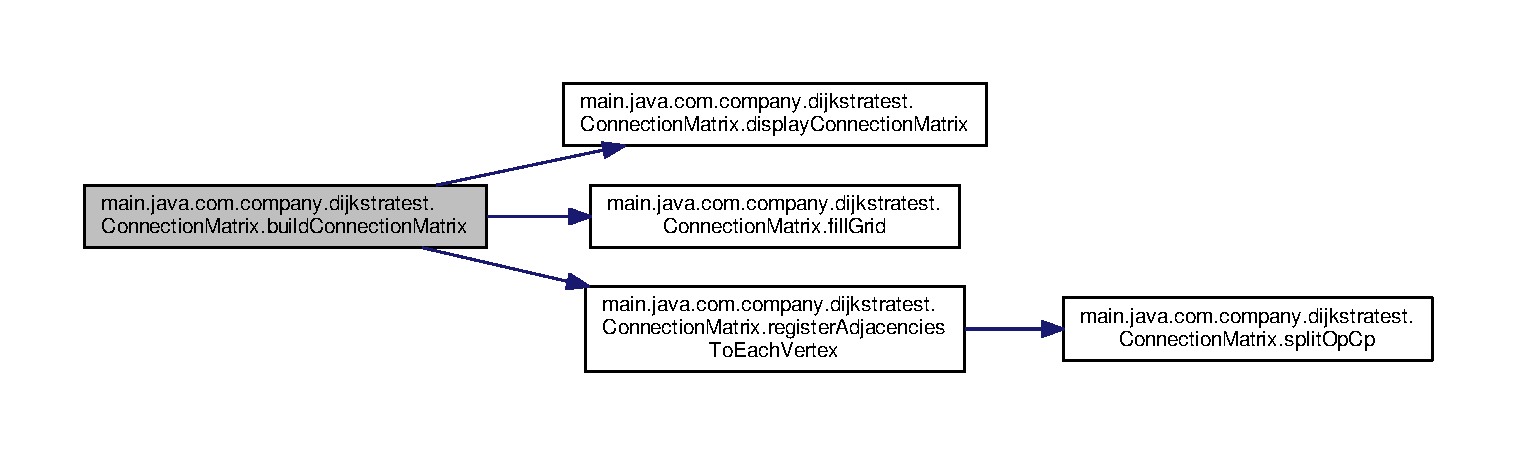
\includegraphics[width=350pt]{classmain_1_1java_1_1com_1_1company_1_1dijkstratest_1_1_connection_matrix_a883880082124638cae78f50746006e5b_cgraph}
\end{center}
\end{figure}


\hypertarget{classmain_1_1java_1_1com_1_1company_1_1dijkstratest_1_1_connection_matrix_ad305dcd4ab25d7628dd843451e1856be}{\index{main\-::java\-::com\-::company\-::dijkstratest\-::\-Connection\-Matrix@{main\-::java\-::com\-::company\-::dijkstratest\-::\-Connection\-Matrix}!display\-Connection\-Matrix@{display\-Connection\-Matrix}}
\index{display\-Connection\-Matrix@{display\-Connection\-Matrix}!main::java::com::company::dijkstratest::ConnectionMatrix@{main\-::java\-::com\-::company\-::dijkstratest\-::\-Connection\-Matrix}}
\subsubsection[{display\-Connection\-Matrix}]{\setlength{\rightskip}{0pt plus 5cm}void main.\-java.\-com.\-company.\-dijkstratest.\-Connection\-Matrix.\-display\-Connection\-Matrix (
\begin{DoxyParamCaption}
{}
\end{DoxyParamCaption}
)}}\label{classmain_1_1java_1_1com_1_1company_1_1dijkstratest_1_1_connection_matrix_ad305dcd4ab25d7628dd843451e1856be}


Definition at line 98 of file Connection\-Matrix.\-java.



References main.\-java.\-com.\-company.\-dijkstratest.\-Connection\-Matrix.\-matrix.



Referenced by main.\-java.\-com.\-company.\-dijkstratest.\-Connection\-Matrix.\-build\-Connection\-Matrix().

\hypertarget{classmain_1_1java_1_1com_1_1company_1_1dijkstratest_1_1_connection_matrix_ab761efa04c328a3362d653a6612dd404}{\index{main\-::java\-::com\-::company\-::dijkstratest\-::\-Connection\-Matrix@{main\-::java\-::com\-::company\-::dijkstratest\-::\-Connection\-Matrix}!fill\-Grid@{fill\-Grid}}
\index{fill\-Grid@{fill\-Grid}!main::java::com::company::dijkstratest::ConnectionMatrix@{main\-::java\-::com\-::company\-::dijkstratest\-::\-Connection\-Matrix}}
\subsubsection[{fill\-Grid}]{\setlength{\rightskip}{0pt plus 5cm}void main.\-java.\-com.\-company.\-dijkstratest.\-Connection\-Matrix.\-fill\-Grid (
\begin{DoxyParamCaption}
{}
\end{DoxyParamCaption}
)}}\label{classmain_1_1java_1_1com_1_1company_1_1dijkstratest_1_1_connection_matrix_ab761efa04c328a3362d653a6612dd404}
Build the Connection matrix base on the choose subscriber's neighborhood info with other subscribers 

Definition at line 77 of file Connection\-Matrix.\-java.



References main.\-java.\-com.\-company.\-dijkstratest.\-Connection\-Matrix.\-vertices.



Referenced by main.\-java.\-com.\-company.\-dijkstratest.\-Connection\-Matrix.\-build\-Connection\-Matrix().

\hypertarget{classmain_1_1java_1_1com_1_1company_1_1dijkstratest_1_1_connection_matrix_ade4179ca5619dadb5a2bbadab52ac93e}{\index{main\-::java\-::com\-::company\-::dijkstratest\-::\-Connection\-Matrix@{main\-::java\-::com\-::company\-::dijkstratest\-::\-Connection\-Matrix}!register\-Adjacencies\-To\-Each\-Vertex@{register\-Adjacencies\-To\-Each\-Vertex}}
\index{register\-Adjacencies\-To\-Each\-Vertex@{register\-Adjacencies\-To\-Each\-Vertex}!main::java::com::company::dijkstratest::ConnectionMatrix@{main\-::java\-::com\-::company\-::dijkstratest\-::\-Connection\-Matrix}}
\subsubsection[{register\-Adjacencies\-To\-Each\-Vertex}]{\setlength{\rightskip}{0pt plus 5cm}void main.\-java.\-com.\-company.\-dijkstratest.\-Connection\-Matrix.\-register\-Adjacencies\-To\-Each\-Vertex (
\begin{DoxyParamCaption}
{}
\end{DoxyParamCaption}
)}}\label{classmain_1_1java_1_1com_1_1company_1_1dijkstratest_1_1_connection_matrix_ade4179ca5619dadb5a2bbadab52ac93e}


Definition at line 37 of file Connection\-Matrix.\-java.



References main.\-java.\-com.\-company.\-dijkstratest.\-Connection\-Matrix.\-adjacency\-List, main.\-java.\-com.\-company.\-dijkstratest.\-Connection\-Matrix.\-split\-Op\-Cp(), and main.\-java.\-com.\-company.\-dijkstratest.\-Connection\-Matrix.\-vertices.



Referenced by main.\-java.\-com.\-company.\-dijkstratest.\-Connection\-Matrix.\-build\-Connection\-Matrix().



Here is the call graph for this function\-:
\nopagebreak
\begin{figure}[H]
\begin{center}
\leavevmode
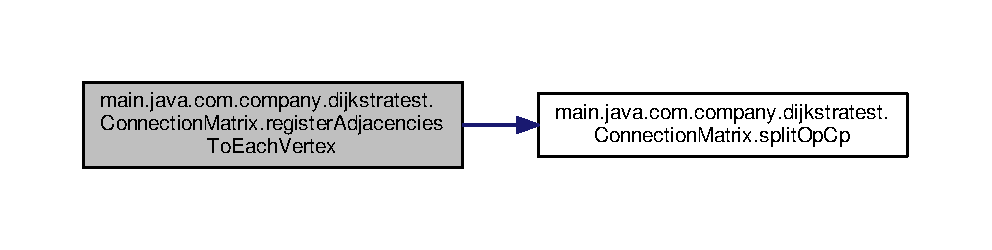
\includegraphics[width=350pt]{classmain_1_1java_1_1com_1_1company_1_1dijkstratest_1_1_connection_matrix_ade4179ca5619dadb5a2bbadab52ac93e_cgraph}
\end{center}
\end{figure}


\hypertarget{classmain_1_1java_1_1com_1_1company_1_1dijkstratest_1_1_connection_matrix_a40c35866fd543064f675971e91a88a75}{\index{main\-::java\-::com\-::company\-::dijkstratest\-::\-Connection\-Matrix@{main\-::java\-::com\-::company\-::dijkstratest\-::\-Connection\-Matrix}!split\-Op\-Cp@{split\-Op\-Cp}}
\index{split\-Op\-Cp@{split\-Op\-Cp}!main::java::com::company::dijkstratest::ConnectionMatrix@{main\-::java\-::com\-::company\-::dijkstratest\-::\-Connection\-Matrix}}
\subsubsection[{split\-Op\-Cp}]{\setlength{\rightskip}{0pt plus 5cm}String \mbox{[}$\,$\mbox{]} main.\-java.\-com.\-company.\-dijkstratest.\-Connection\-Matrix.\-split\-Op\-Cp (
\begin{DoxyParamCaption}
\item[{String}]{op\-Cp}
\end{DoxyParamCaption}
)}}\label{classmain_1_1java_1_1com_1_1company_1_1dijkstratest_1_1_connection_matrix_a40c35866fd543064f675971e91a88a75}
Split the \char`\"{}op-\/cp\char`\"{} form, and put op and cp into an array


\begin{DoxyParams}{Parameters}
{\em op\-Cp} & the \char`\"{}op-\/cp\char`\"{} String \\
\hline
\end{DoxyParams}
\begin{DoxyReturn}{Returns}
an array holds both op and cp 
\end{DoxyReturn}


Definition at line 67 of file Connection\-Matrix.\-java.



Referenced by main.\-java.\-com.\-company.\-dijkstratest.\-Connection\-Matrix.\-register\-Adjacencies\-To\-Each\-Vertex().



\subsection{Member Data Documentation}
\hypertarget{classmain_1_1java_1_1com_1_1company_1_1dijkstratest_1_1_connection_matrix_a0fcd8b3828105bd570fd97dca77db1ea}{\index{main\-::java\-::com\-::company\-::dijkstratest\-::\-Connection\-Matrix@{main\-::java\-::com\-::company\-::dijkstratest\-::\-Connection\-Matrix}!adjacency\-List@{adjacency\-List}}
\index{adjacency\-List@{adjacency\-List}!main::java::com::company::dijkstratest::ConnectionMatrix@{main\-::java\-::com\-::company\-::dijkstratest\-::\-Connection\-Matrix}}
\subsubsection[{adjacency\-List}]{\setlength{\rightskip}{0pt plus 5cm}final Array\-List$<$String$>$ main.\-java.\-com.\-company.\-dijkstratest.\-Connection\-Matrix.\-adjacency\-List\hspace{0.3cm}{\ttfamily [private]}}}\label{classmain_1_1java_1_1com_1_1company_1_1dijkstratest_1_1_connection_matrix_a0fcd8b3828105bd570fd97dca77db1ea}


Definition at line 13 of file Connection\-Matrix.\-java.



Referenced by main.\-java.\-com.\-company.\-dijkstratest.\-Connection\-Matrix.\-Connection\-Matrix(), and main.\-java.\-com.\-company.\-dijkstratest.\-Connection\-Matrix.\-register\-Adjacencies\-To\-Each\-Vertex().

\hypertarget{classmain_1_1java_1_1com_1_1company_1_1dijkstratest_1_1_connection_matrix_a3c077791f0b8164d8c19f67d250f43fd}{\index{main\-::java\-::com\-::company\-::dijkstratest\-::\-Connection\-Matrix@{main\-::java\-::com\-::company\-::dijkstratest\-::\-Connection\-Matrix}!matrix@{matrix}}
\index{matrix@{matrix}!main::java::com::company::dijkstratest::ConnectionMatrix@{main\-::java\-::com\-::company\-::dijkstratest\-::\-Connection\-Matrix}}
\subsubsection[{matrix}]{\setlength{\rightskip}{0pt plus 5cm}final Array\-List$<$Array\-List$<$Integer$>$ $>$ main.\-java.\-com.\-company.\-dijkstratest.\-Connection\-Matrix.\-matrix = new Array\-List$<$Array\-List$<$Integer$>$$>$()\hspace{0.3cm}{\ttfamily [private]}}}\label{classmain_1_1java_1_1com_1_1company_1_1dijkstratest_1_1_connection_matrix_a3c077791f0b8164d8c19f67d250f43fd}


Definition at line 15 of file Connection\-Matrix.\-java.



Referenced by main.\-java.\-com.\-company.\-dijkstratest.\-Connection\-Matrix.\-display\-Connection\-Matrix().

\hypertarget{classmain_1_1java_1_1com_1_1company_1_1dijkstratest_1_1_connection_matrix_a372aa9baecc703f490a3eef8845bc7a7}{\index{main\-::java\-::com\-::company\-::dijkstratest\-::\-Connection\-Matrix@{main\-::java\-::com\-::company\-::dijkstratest\-::\-Connection\-Matrix}!vertices@{vertices}}
\index{vertices@{vertices}!main::java::com::company::dijkstratest::ConnectionMatrix@{main\-::java\-::com\-::company\-::dijkstratest\-::\-Connection\-Matrix}}
\subsubsection[{vertices}]{\setlength{\rightskip}{0pt plus 5cm}final Array\-List$<${\bf Vertex}$>$ main.\-java.\-com.\-company.\-dijkstratest.\-Connection\-Matrix.\-vertices\hspace{0.3cm}{\ttfamily [private]}}}\label{classmain_1_1java_1_1com_1_1company_1_1dijkstratest_1_1_connection_matrix_a372aa9baecc703f490a3eef8845bc7a7}


Definition at line 14 of file Connection\-Matrix.\-java.



Referenced by main.\-java.\-com.\-company.\-dijkstratest.\-Connection\-Matrix.\-Connection\-Matrix(), main.\-java.\-com.\-company.\-dijkstratest.\-Connection\-Matrix.\-fill\-Grid(), and main.\-java.\-com.\-company.\-dijkstratest.\-Connection\-Matrix.\-register\-Adjacencies\-To\-Each\-Vertex().



The documentation for this class was generated from the following file\-:\begin{DoxyCompactItemize}
\item 
src/main/java/com/company/dijkstratest/\hyperlink{_connection_matrix_8java}{Connection\-Matrix.\-java}\end{DoxyCompactItemize}

\hypertarget{class_dijkstra}{\section{Dijkstra Class Reference}
\label{class_dijkstra}\index{Dijkstra@{Dijkstra}}
}
\subsection*{Static Public Member Functions}
\begin{DoxyCompactItemize}
\item 
static void \hyperlink{class_dijkstra_a0ae42b709899e084d6910727ef0da3fd}{compute\-Paths} (Vertex source)
\item 
static List$<$ Vertex $>$ \hyperlink{class_dijkstra_a76b0c0b81ad3157dd93d4038b35906ae}{get\-Shortest\-Path\-To} (Vertex target)
\item 
static void \hyperlink{class_dijkstra_a8be51d89fb674d80b69a75bba223d529}{main} (String\mbox{[}$\,$\mbox{]} args)
\end{DoxyCompactItemize}


\subsection{Detailed Description}


Definition at line 56 of file Dijkstra.\-java.



\subsection{Member Function Documentation}
\hypertarget{class_dijkstra_a0ae42b709899e084d6910727ef0da3fd}{\index{Dijkstra@{Dijkstra}!compute\-Paths@{compute\-Paths}}
\index{compute\-Paths@{compute\-Paths}!Dijkstra@{Dijkstra}}
\subsubsection[{compute\-Paths}]{\setlength{\rightskip}{0pt plus 5cm}static void Dijkstra.\-compute\-Paths (
\begin{DoxyParamCaption}
\item[{Vertex}]{source}
\end{DoxyParamCaption}
)\hspace{0.3cm}{\ttfamily [static]}}}\label{class_dijkstra_a0ae42b709899e084d6910727ef0da3fd}


Definition at line 58 of file Dijkstra.\-java.



Referenced by main().

\hypertarget{class_dijkstra_a76b0c0b81ad3157dd93d4038b35906ae}{\index{Dijkstra@{Dijkstra}!get\-Shortest\-Path\-To@{get\-Shortest\-Path\-To}}
\index{get\-Shortest\-Path\-To@{get\-Shortest\-Path\-To}!Dijkstra@{Dijkstra}}
\subsubsection[{get\-Shortest\-Path\-To}]{\setlength{\rightskip}{0pt plus 5cm}static List$<$Vertex$>$ Dijkstra.\-get\-Shortest\-Path\-To (
\begin{DoxyParamCaption}
\item[{Vertex}]{target}
\end{DoxyParamCaption}
)\hspace{0.3cm}{\ttfamily [static]}}}\label{class_dijkstra_a76b0c0b81ad3157dd93d4038b35906ae}


Definition at line 84 of file Dijkstra.\-java.



Referenced by main().

\hypertarget{class_dijkstra_a8be51d89fb674d80b69a75bba223d529}{\index{Dijkstra@{Dijkstra}!main@{main}}
\index{main@{main}!Dijkstra@{Dijkstra}}
\subsubsection[{main}]{\setlength{\rightskip}{0pt plus 5cm}static void Dijkstra.\-main (
\begin{DoxyParamCaption}
\item[{String\mbox{[}$\,$\mbox{]}}]{args}
\end{DoxyParamCaption}
)\hspace{0.3cm}{\ttfamily [static]}}}\label{class_dijkstra_a8be51d89fb674d80b69a75bba223d529}


Definition at line 94 of file Dijkstra.\-java.



References compute\-Paths(), and get\-Shortest\-Path\-To().



Here is the call graph for this function\-:
\nopagebreak
\begin{figure}[H]
\begin{center}
\leavevmode
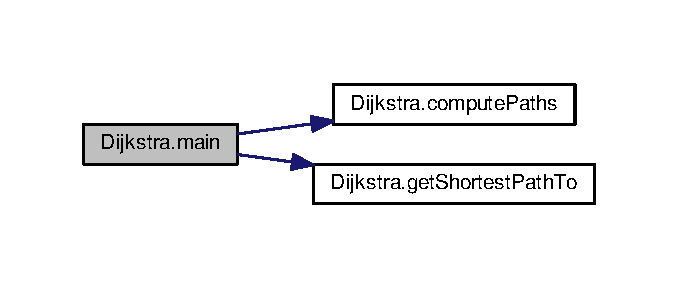
\includegraphics[width=326pt]{class_dijkstra_a8be51d89fb674d80b69a75bba223d529_cgraph}
\end{center}
\end{figure}




The documentation for this class was generated from the following file\-:\begin{DoxyCompactItemize}
\item 
help/\hyperlink{_dijkstra_8java}{Dijkstra.\-java}\end{DoxyCompactItemize}

\hypertarget{classmain_1_1java_1_1com_1_1company_1_1dijkstratest_1_1_main}{\section{main.\-java.\-com.\-company.\-dijkstratest.\-Main Class Reference}
\label{classmain_1_1java_1_1com_1_1company_1_1dijkstratest_1_1_main}\index{main.\-java.\-com.\-company.\-dijkstratest.\-Main@{main.\-java.\-com.\-company.\-dijkstratest.\-Main}}
}


Collaboration diagram for main.\-java.\-com.\-company.\-dijkstratest.\-Main\-:
\nopagebreak
\begin{figure}[H]
\begin{center}
\leavevmode
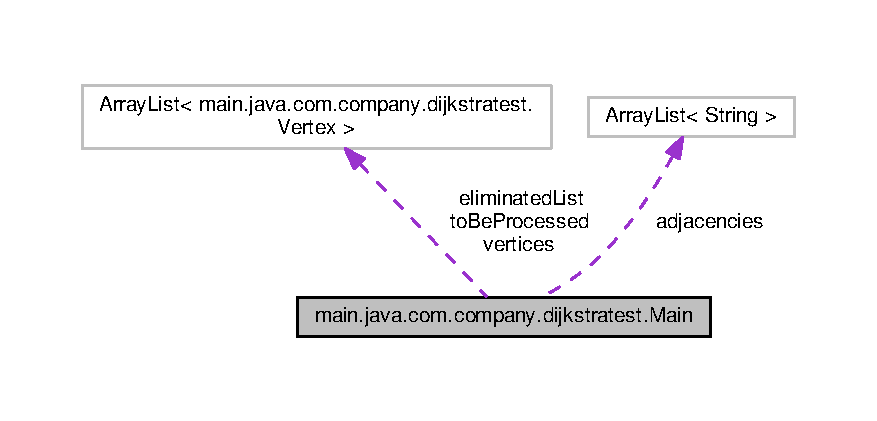
\includegraphics[width=350pt]{classmain_1_1java_1_1com_1_1company_1_1dijkstratest_1_1_main__coll__graph}
\end{center}
\end{figure}
\subsection*{Public Member Functions}
\begin{DoxyCompactItemize}
\item 
void \hyperlink{classmain_1_1java_1_1com_1_1company_1_1dijkstratest_1_1_main_aecef650b770eeab79fb0620dee263f77}{go} (String\mbox{[}$\,$\mbox{]} args)
\item 
void \hyperlink{classmain_1_1java_1_1com_1_1company_1_1dijkstratest_1_1_main_a3e5569d3503edf65388ea1b8fad02742}{display\-Prefix} ()
\end{DoxyCompactItemize}
\subsection*{Static Public Member Functions}
\begin{DoxyCompactItemize}
\item 
static void \hyperlink{classmain_1_1java_1_1com_1_1company_1_1dijkstratest_1_1_main_a41add3527abb4fb4d0c9640aa20fba59}{main} (String\mbox{[}$\,$\mbox{]} args)
\end{DoxyCompactItemize}
\subsection*{Private Attributes}
\begin{DoxyCompactItemize}
\item 
Array\-List$<$ String $>$ \hyperlink{classmain_1_1java_1_1com_1_1company_1_1dijkstratest_1_1_main_a0d4996e719ec846ccd4be7d21cdfb2e5}{adjacencies} = new Array\-List$<$String$>$()
\item 
Array\-List$<$ \hyperlink{classmain_1_1java_1_1com_1_1company_1_1dijkstratest_1_1_vertex}{Vertex} $>$ \hyperlink{classmain_1_1java_1_1com_1_1company_1_1dijkstratest_1_1_main_a9e9e1529522bffb58584b4f319e07217}{vertices} = new Array\-List$<$\hyperlink{classmain_1_1java_1_1com_1_1company_1_1dijkstratest_1_1_vertex}{Vertex}$>$()
\item 
Array\-List$<$ \hyperlink{classmain_1_1java_1_1com_1_1company_1_1dijkstratest_1_1_vertex}{Vertex} $>$ \hyperlink{classmain_1_1java_1_1com_1_1company_1_1dijkstratest_1_1_main_a557eccaa4afe7d83cf6cc262d1ba1f3d}{to\-Be\-Processed} = new Array\-List$<$\hyperlink{classmain_1_1java_1_1com_1_1company_1_1dijkstratest_1_1_vertex}{Vertex}$>$()
\item 
Array\-List$<$ \hyperlink{classmain_1_1java_1_1com_1_1company_1_1dijkstratest_1_1_vertex}{Vertex} $>$ \hyperlink{classmain_1_1java_1_1com_1_1company_1_1dijkstratest_1_1_main_af031de92d898217502e31dcd4d6c9539}{eliminated\-List} = new Array\-List$<$\hyperlink{classmain_1_1java_1_1com_1_1company_1_1dijkstratest_1_1_vertex}{Vertex}$>$()
\end{DoxyCompactItemize}


\subsection{Detailed Description}
\begin{DoxyAuthor}{Author}
hzhang 
\end{DoxyAuthor}


Definition at line 11 of file Main.\-java.



\subsection{Member Function Documentation}
\hypertarget{classmain_1_1java_1_1com_1_1company_1_1dijkstratest_1_1_main_a3e5569d3503edf65388ea1b8fad02742}{\index{main\-::java\-::com\-::company\-::dijkstratest\-::\-Main@{main\-::java\-::com\-::company\-::dijkstratest\-::\-Main}!display\-Prefix@{display\-Prefix}}
\index{display\-Prefix@{display\-Prefix}!main::java::com::company::dijkstratest::Main@{main\-::java\-::com\-::company\-::dijkstratest\-::\-Main}}
\subsubsection[{display\-Prefix}]{\setlength{\rightskip}{0pt plus 5cm}void main.\-java.\-com.\-company.\-dijkstratest.\-Main.\-display\-Prefix (
\begin{DoxyParamCaption}
{}
\end{DoxyParamCaption}
)}}\label{classmain_1_1java_1_1com_1_1company_1_1dijkstratest_1_1_main_a3e5569d3503edf65388ea1b8fad02742}
Print the prefix row 

Definition at line 69 of file Main.\-java.



References main.\-java.\-com.\-company.\-dijkstratest.\-Main.\-vertices.

\hypertarget{classmain_1_1java_1_1com_1_1company_1_1dijkstratest_1_1_main_aecef650b770eeab79fb0620dee263f77}{\index{main\-::java\-::com\-::company\-::dijkstratest\-::\-Main@{main\-::java\-::com\-::company\-::dijkstratest\-::\-Main}!go@{go}}
\index{go@{go}!main::java::com::company::dijkstratest::Main@{main\-::java\-::com\-::company\-::dijkstratest\-::\-Main}}
\subsubsection[{go}]{\setlength{\rightskip}{0pt plus 5cm}void main.\-java.\-com.\-company.\-dijkstratest.\-Main.\-go (
\begin{DoxyParamCaption}
\item[{String\mbox{[}$\,$\mbox{]}}]{args}
\end{DoxyParamCaption}
)}}\label{classmain_1_1java_1_1com_1_1company_1_1dijkstratest_1_1_main_aecef650b770eeab79fb0620dee263f77}


Definition at line 24 of file Main.\-java.



References main.\-java.\-com.\-company.\-dijkstratest.\-Main.\-adjacencies, main.\-java.\-com.\-company.\-dijkstratest.\-Main.\-eliminated\-List, main.\-java.\-com.\-company.\-dijkstratest.\-Main.\-to\-Be\-Processed, and main.\-java.\-com.\-company.\-dijkstratest.\-Main.\-vertices.

\hypertarget{classmain_1_1java_1_1com_1_1company_1_1dijkstratest_1_1_main_a41add3527abb4fb4d0c9640aa20fba59}{\index{main\-::java\-::com\-::company\-::dijkstratest\-::\-Main@{main\-::java\-::com\-::company\-::dijkstratest\-::\-Main}!main@{main}}
\index{main@{main}!main::java::com::company::dijkstratest::Main@{main\-::java\-::com\-::company\-::dijkstratest\-::\-Main}}
\subsubsection[{main}]{\setlength{\rightskip}{0pt plus 5cm}static void main.\-java.\-com.\-company.\-dijkstratest.\-Main.\-main (
\begin{DoxyParamCaption}
\item[{String\mbox{[}$\,$\mbox{]}}]{args}
\end{DoxyParamCaption}
)\hspace{0.3cm}{\ttfamily [static]}}}\label{classmain_1_1java_1_1com_1_1company_1_1dijkstratest_1_1_main_a41add3527abb4fb4d0c9640aa20fba59}


Definition at line 18 of file Main.\-java.



\subsection{Member Data Documentation}
\hypertarget{classmain_1_1java_1_1com_1_1company_1_1dijkstratest_1_1_main_a0d4996e719ec846ccd4be7d21cdfb2e5}{\index{main\-::java\-::com\-::company\-::dijkstratest\-::\-Main@{main\-::java\-::com\-::company\-::dijkstratest\-::\-Main}!adjacencies@{adjacencies}}
\index{adjacencies@{adjacencies}!main::java::com::company::dijkstratest::Main@{main\-::java\-::com\-::company\-::dijkstratest\-::\-Main}}
\subsubsection[{adjacencies}]{\setlength{\rightskip}{0pt plus 5cm}Array\-List$<$String$>$ main.\-java.\-com.\-company.\-dijkstratest.\-Main.\-adjacencies = new Array\-List$<$String$>$()\hspace{0.3cm}{\ttfamily [private]}}}\label{classmain_1_1java_1_1com_1_1company_1_1dijkstratest_1_1_main_a0d4996e719ec846ccd4be7d21cdfb2e5}


Definition at line 13 of file Main.\-java.



Referenced by main.\-java.\-com.\-company.\-dijkstratest.\-Main.\-go().

\hypertarget{classmain_1_1java_1_1com_1_1company_1_1dijkstratest_1_1_main_af031de92d898217502e31dcd4d6c9539}{\index{main\-::java\-::com\-::company\-::dijkstratest\-::\-Main@{main\-::java\-::com\-::company\-::dijkstratest\-::\-Main}!eliminated\-List@{eliminated\-List}}
\index{eliminated\-List@{eliminated\-List}!main::java::com::company::dijkstratest::Main@{main\-::java\-::com\-::company\-::dijkstratest\-::\-Main}}
\subsubsection[{eliminated\-List}]{\setlength{\rightskip}{0pt plus 5cm}Array\-List$<${\bf Vertex}$>$ main.\-java.\-com.\-company.\-dijkstratest.\-Main.\-eliminated\-List = new Array\-List$<${\bf Vertex}$>$()\hspace{0.3cm}{\ttfamily [private]}}}\label{classmain_1_1java_1_1com_1_1company_1_1dijkstratest_1_1_main_af031de92d898217502e31dcd4d6c9539}


Definition at line 16 of file Main.\-java.



Referenced by main.\-java.\-com.\-company.\-dijkstratest.\-Main.\-go().

\hypertarget{classmain_1_1java_1_1com_1_1company_1_1dijkstratest_1_1_main_a557eccaa4afe7d83cf6cc262d1ba1f3d}{\index{main\-::java\-::com\-::company\-::dijkstratest\-::\-Main@{main\-::java\-::com\-::company\-::dijkstratest\-::\-Main}!to\-Be\-Processed@{to\-Be\-Processed}}
\index{to\-Be\-Processed@{to\-Be\-Processed}!main::java::com::company::dijkstratest::Main@{main\-::java\-::com\-::company\-::dijkstratest\-::\-Main}}
\subsubsection[{to\-Be\-Processed}]{\setlength{\rightskip}{0pt plus 5cm}Array\-List$<${\bf Vertex}$>$ main.\-java.\-com.\-company.\-dijkstratest.\-Main.\-to\-Be\-Processed = new Array\-List$<${\bf Vertex}$>$()\hspace{0.3cm}{\ttfamily [private]}}}\label{classmain_1_1java_1_1com_1_1company_1_1dijkstratest_1_1_main_a557eccaa4afe7d83cf6cc262d1ba1f3d}


Definition at line 15 of file Main.\-java.



Referenced by main.\-java.\-com.\-company.\-dijkstratest.\-Main.\-go().

\hypertarget{classmain_1_1java_1_1com_1_1company_1_1dijkstratest_1_1_main_a9e9e1529522bffb58584b4f319e07217}{\index{main\-::java\-::com\-::company\-::dijkstratest\-::\-Main@{main\-::java\-::com\-::company\-::dijkstratest\-::\-Main}!vertices@{vertices}}
\index{vertices@{vertices}!main::java::com::company::dijkstratest::Main@{main\-::java\-::com\-::company\-::dijkstratest\-::\-Main}}
\subsubsection[{vertices}]{\setlength{\rightskip}{0pt plus 5cm}Array\-List$<${\bf Vertex}$>$ main.\-java.\-com.\-company.\-dijkstratest.\-Main.\-vertices = new Array\-List$<${\bf Vertex}$>$()\hspace{0.3cm}{\ttfamily [private]}}}\label{classmain_1_1java_1_1com_1_1company_1_1dijkstratest_1_1_main_a9e9e1529522bffb58584b4f319e07217}


Definition at line 14 of file Main.\-java.



Referenced by main.\-java.\-com.\-company.\-dijkstratest.\-Main.\-display\-Prefix(), and main.\-java.\-com.\-company.\-dijkstratest.\-Main.\-go().



The documentation for this class was generated from the following file\-:\begin{DoxyCompactItemize}
\item 
src/main/java/com/company/dijkstratest/\hyperlink{_main_8java}{Main.\-java}\end{DoxyCompactItemize}

\hypertarget{classmain_1_1java_1_1com_1_1company_1_1dijkstratest_1_1_pair}{\section{main.\-java.\-com.\-company.\-dijkstratest.\-Pair Class Reference}
\label{classmain_1_1java_1_1com_1_1company_1_1dijkstratest_1_1_pair}\index{main.\-java.\-com.\-company.\-dijkstratest.\-Pair@{main.\-java.\-com.\-company.\-dijkstratest.\-Pair}}
}


Inheritance diagram for main.\-java.\-com.\-company.\-dijkstratest.\-Pair\-:
\nopagebreak
\begin{figure}[H]
\begin{center}
\leavevmode
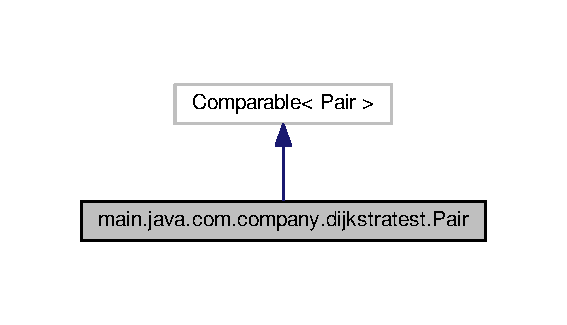
\includegraphics[width=272pt]{classmain_1_1java_1_1com_1_1company_1_1dijkstratest_1_1_pair__inherit__graph}
\end{center}
\end{figure}


Collaboration diagram for main.\-java.\-com.\-company.\-dijkstratest.\-Pair\-:
\nopagebreak
\begin{figure}[H]
\begin{center}
\leavevmode
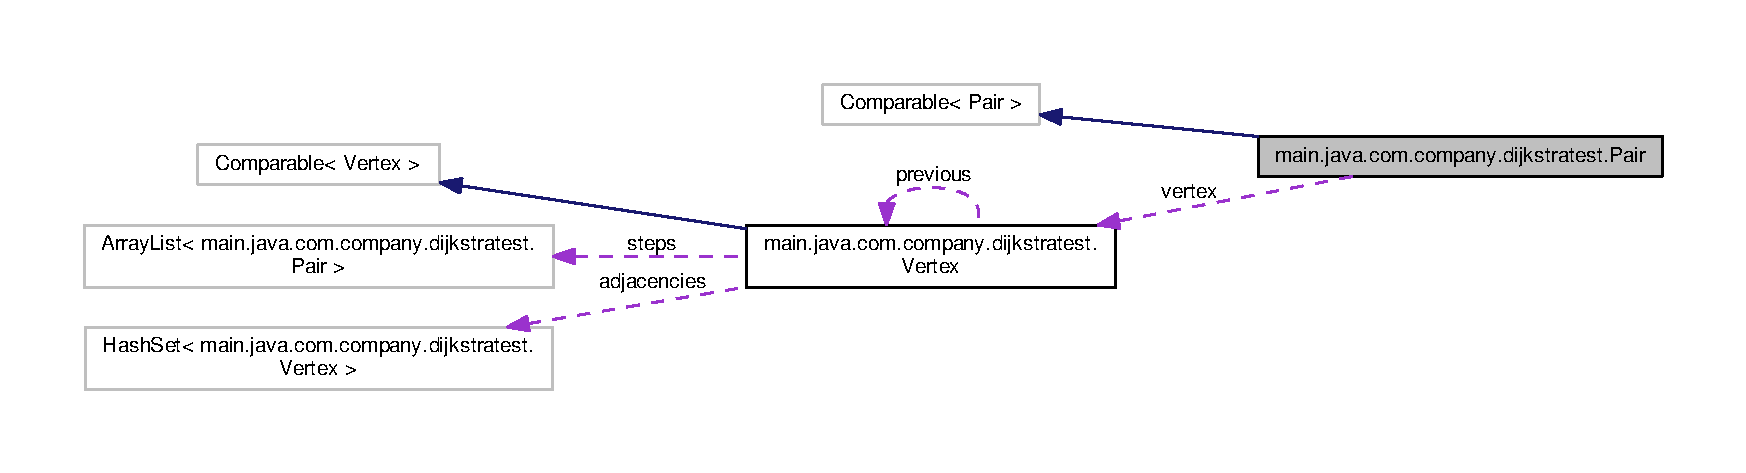
\includegraphics[width=350pt]{classmain_1_1java_1_1com_1_1company_1_1dijkstratest_1_1_pair__coll__graph}
\end{center}
\end{figure}
\subsection*{Public Member Functions}
\begin{DoxyCompactItemize}
\item 
\hyperlink{classmain_1_1java_1_1com_1_1company_1_1dijkstratest_1_1_pair_a211595a122698caf689814de3104723b}{Pair} (\hyperlink{classmain_1_1java_1_1com_1_1company_1_1dijkstratest_1_1_vertex}{Vertex} v, int s)
\item 
\hyperlink{classmain_1_1java_1_1com_1_1company_1_1dijkstratest_1_1_vertex}{Vertex} \hyperlink{classmain_1_1java_1_1com_1_1company_1_1dijkstratest_1_1_pair_a84296cc6eaa19d0f50f8ca98a7c98639}{get\-Vertex} ()
\item 
void \hyperlink{classmain_1_1java_1_1com_1_1company_1_1dijkstratest_1_1_pair_aede90e0406606c28b1565dafcf2cedda}{set\-Step\-Number\-To\-Infinity} ()
\item 
int \hyperlink{classmain_1_1java_1_1com_1_1company_1_1dijkstratest_1_1_pair_a05b2374c70c937227f898b1cea0fe910}{get\-Step\-Number} ()
\item 
int \hyperlink{classmain_1_1java_1_1com_1_1company_1_1dijkstratest_1_1_pair_adf087853df8cae9edc2c5b206e98a740}{compare\-To} (\hyperlink{classmain_1_1java_1_1com_1_1company_1_1dijkstratest_1_1_pair}{Pair} other)
\end{DoxyCompactItemize}
\subsection*{Private Attributes}
\begin{DoxyCompactItemize}
\item 
\hyperlink{classmain_1_1java_1_1com_1_1company_1_1dijkstratest_1_1_vertex}{Vertex} \hyperlink{classmain_1_1java_1_1com_1_1company_1_1dijkstratest_1_1_pair_a1060ef3a7196fae57fde28c911ad02a0}{vertex}
\item 
int \hyperlink{classmain_1_1java_1_1com_1_1company_1_1dijkstratest_1_1_pair_a4bc5c040004202d37e76798124cb1624}{step\-Number}
\end{DoxyCompactItemize}


\subsection{Detailed Description}
\hyperlink{classmain_1_1java_1_1com_1_1company_1_1dijkstratest_1_1_pair}{Pair} hold vertex and the steps from the vertex to all others \begin{DoxyAuthor}{Author}
hzhang 
\end{DoxyAuthor}


Definition at line 7 of file Pair.\-java.



\subsection{Constructor \& Destructor Documentation}
\hypertarget{classmain_1_1java_1_1com_1_1company_1_1dijkstratest_1_1_pair_a211595a122698caf689814de3104723b}{\index{main\-::java\-::com\-::company\-::dijkstratest\-::\-Pair@{main\-::java\-::com\-::company\-::dijkstratest\-::\-Pair}!Pair@{Pair}}
\index{Pair@{Pair}!main::java::com::company::dijkstratest::Pair@{main\-::java\-::com\-::company\-::dijkstratest\-::\-Pair}}
\subsubsection[{Pair}]{\setlength{\rightskip}{0pt plus 5cm}main.\-java.\-com.\-company.\-dijkstratest.\-Pair.\-Pair (
\begin{DoxyParamCaption}
\item[{{\bf Vertex}}]{v, }
\item[{int}]{s}
\end{DoxyParamCaption}
)}}\label{classmain_1_1java_1_1com_1_1company_1_1dijkstratest_1_1_pair_a211595a122698caf689814de3104723b}


Definition at line 12 of file Pair.\-java.



\subsection{Member Function Documentation}
\hypertarget{classmain_1_1java_1_1com_1_1company_1_1dijkstratest_1_1_pair_adf087853df8cae9edc2c5b206e98a740}{\index{main\-::java\-::com\-::company\-::dijkstratest\-::\-Pair@{main\-::java\-::com\-::company\-::dijkstratest\-::\-Pair}!compare\-To@{compare\-To}}
\index{compare\-To@{compare\-To}!main::java::com::company::dijkstratest::Pair@{main\-::java\-::com\-::company\-::dijkstratest\-::\-Pair}}
\subsubsection[{compare\-To}]{\setlength{\rightskip}{0pt plus 5cm}int main.\-java.\-com.\-company.\-dijkstratest.\-Pair.\-compare\-To (
\begin{DoxyParamCaption}
\item[{{\bf Pair}}]{other}
\end{DoxyParamCaption}
)}}\label{classmain_1_1java_1_1com_1_1company_1_1dijkstratest_1_1_pair_adf087853df8cae9edc2c5b206e98a740}
Sort \hyperlink{classmain_1_1java_1_1com_1_1company_1_1dijkstratest_1_1_pair}{Pair} object 
\begin{DoxyParams}{Parameters}
{\em other} & \\
\hline
\end{DoxyParams}
\begin{DoxyReturn}{Returns}

\end{DoxyReturn}


Definition at line 38 of file Pair.\-java.



References main.\-java.\-com.\-company.\-dijkstratest.\-Pair.\-get\-Step\-Number(), and main.\-java.\-com.\-company.\-dijkstratest.\-Pair.\-get\-Vertex().



Here is the call graph for this function\-:
\nopagebreak
\begin{figure}[H]
\begin{center}
\leavevmode
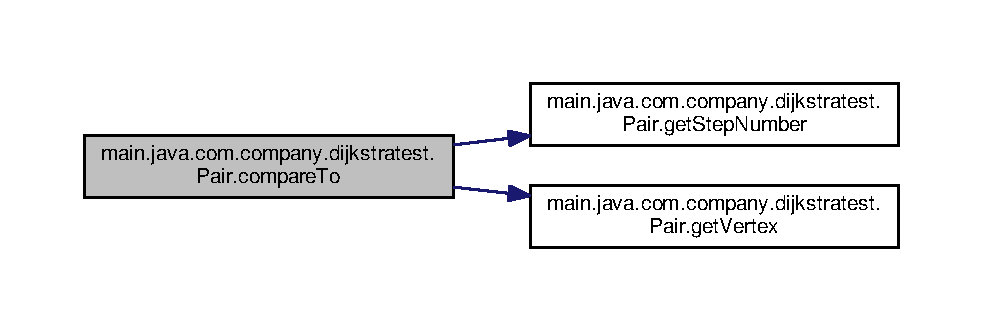
\includegraphics[width=350pt]{classmain_1_1java_1_1com_1_1company_1_1dijkstratest_1_1_pair_adf087853df8cae9edc2c5b206e98a740_cgraph}
\end{center}
\end{figure}


\hypertarget{classmain_1_1java_1_1com_1_1company_1_1dijkstratest_1_1_pair_a05b2374c70c937227f898b1cea0fe910}{\index{main\-::java\-::com\-::company\-::dijkstratest\-::\-Pair@{main\-::java\-::com\-::company\-::dijkstratest\-::\-Pair}!get\-Step\-Number@{get\-Step\-Number}}
\index{get\-Step\-Number@{get\-Step\-Number}!main::java::com::company::dijkstratest::Pair@{main\-::java\-::com\-::company\-::dijkstratest\-::\-Pair}}
\subsubsection[{get\-Step\-Number}]{\setlength{\rightskip}{0pt plus 5cm}int main.\-java.\-com.\-company.\-dijkstratest.\-Pair.\-get\-Step\-Number (
\begin{DoxyParamCaption}
{}
\end{DoxyParamCaption}
)}}\label{classmain_1_1java_1_1com_1_1company_1_1dijkstratest_1_1_pair_a05b2374c70c937227f898b1cea0fe910}


Definition at line 28 of file Pair.\-java.



References main.\-java.\-com.\-company.\-dijkstratest.\-Pair.\-step\-Number.



Referenced by main.\-java.\-com.\-company.\-dijkstratest.\-Pair.\-compare\-To().

\hypertarget{classmain_1_1java_1_1com_1_1company_1_1dijkstratest_1_1_pair_a84296cc6eaa19d0f50f8ca98a7c98639}{\index{main\-::java\-::com\-::company\-::dijkstratest\-::\-Pair@{main\-::java\-::com\-::company\-::dijkstratest\-::\-Pair}!get\-Vertex@{get\-Vertex}}
\index{get\-Vertex@{get\-Vertex}!main::java::com::company::dijkstratest::Pair@{main\-::java\-::com\-::company\-::dijkstratest\-::\-Pair}}
\subsubsection[{get\-Vertex}]{\setlength{\rightskip}{0pt plus 5cm}{\bf Vertex} main.\-java.\-com.\-company.\-dijkstratest.\-Pair.\-get\-Vertex (
\begin{DoxyParamCaption}
{}
\end{DoxyParamCaption}
)}}\label{classmain_1_1java_1_1com_1_1company_1_1dijkstratest_1_1_pair_a84296cc6eaa19d0f50f8ca98a7c98639}


Definition at line 18 of file Pair.\-java.



References main.\-java.\-com.\-company.\-dijkstratest.\-Pair.\-vertex.



Referenced by main.\-java.\-com.\-company.\-dijkstratest.\-Pair.\-compare\-To().

\hypertarget{classmain_1_1java_1_1com_1_1company_1_1dijkstratest_1_1_pair_aede90e0406606c28b1565dafcf2cedda}{\index{main\-::java\-::com\-::company\-::dijkstratest\-::\-Pair@{main\-::java\-::com\-::company\-::dijkstratest\-::\-Pair}!set\-Step\-Number\-To\-Infinity@{set\-Step\-Number\-To\-Infinity}}
\index{set\-Step\-Number\-To\-Infinity@{set\-Step\-Number\-To\-Infinity}!main::java::com::company::dijkstratest::Pair@{main\-::java\-::com\-::company\-::dijkstratest\-::\-Pair}}
\subsubsection[{set\-Step\-Number\-To\-Infinity}]{\setlength{\rightskip}{0pt plus 5cm}void main.\-java.\-com.\-company.\-dijkstratest.\-Pair.\-set\-Step\-Number\-To\-Infinity (
\begin{DoxyParamCaption}
{}
\end{DoxyParamCaption}
)}}\label{classmain_1_1java_1_1com_1_1company_1_1dijkstratest_1_1_pair_aede90e0406606c28b1565dafcf2cedda}


Definition at line 23 of file Pair.\-java.



References main.\-java.\-com.\-company.\-dijkstratest.\-Pair.\-step\-Number.



\subsection{Member Data Documentation}
\hypertarget{classmain_1_1java_1_1com_1_1company_1_1dijkstratest_1_1_pair_a4bc5c040004202d37e76798124cb1624}{\index{main\-::java\-::com\-::company\-::dijkstratest\-::\-Pair@{main\-::java\-::com\-::company\-::dijkstratest\-::\-Pair}!step\-Number@{step\-Number}}
\index{step\-Number@{step\-Number}!main::java::com::company::dijkstratest::Pair@{main\-::java\-::com\-::company\-::dijkstratest\-::\-Pair}}
\subsubsection[{step\-Number}]{\setlength{\rightskip}{0pt plus 5cm}int main.\-java.\-com.\-company.\-dijkstratest.\-Pair.\-step\-Number\hspace{0.3cm}{\ttfamily [private]}}}\label{classmain_1_1java_1_1com_1_1company_1_1dijkstratest_1_1_pair_a4bc5c040004202d37e76798124cb1624}


Definition at line 10 of file Pair.\-java.



Referenced by main.\-java.\-com.\-company.\-dijkstratest.\-Pair.\-get\-Step\-Number(), and main.\-java.\-com.\-company.\-dijkstratest.\-Pair.\-set\-Step\-Number\-To\-Infinity().

\hypertarget{classmain_1_1java_1_1com_1_1company_1_1dijkstratest_1_1_pair_a1060ef3a7196fae57fde28c911ad02a0}{\index{main\-::java\-::com\-::company\-::dijkstratest\-::\-Pair@{main\-::java\-::com\-::company\-::dijkstratest\-::\-Pair}!vertex@{vertex}}
\index{vertex@{vertex}!main::java::com::company::dijkstratest::Pair@{main\-::java\-::com\-::company\-::dijkstratest\-::\-Pair}}
\subsubsection[{vertex}]{\setlength{\rightskip}{0pt plus 5cm}{\bf Vertex} main.\-java.\-com.\-company.\-dijkstratest.\-Pair.\-vertex\hspace{0.3cm}{\ttfamily [private]}}}\label{classmain_1_1java_1_1com_1_1company_1_1dijkstratest_1_1_pair_a1060ef3a7196fae57fde28c911ad02a0}


Definition at line 9 of file Pair.\-java.



Referenced by main.\-java.\-com.\-company.\-dijkstratest.\-Pair.\-get\-Vertex().



The documentation for this class was generated from the following file\-:\begin{DoxyCompactItemize}
\item 
src/main/java/com/company/dijkstratest/\hyperlink{_pair_8java}{Pair.\-java}\end{DoxyCompactItemize}

\hypertarget{classmain_1_1java_1_1com_1_1company_1_1dijkstratest_1_1_registration}{\section{main.\-java.\-com.\-company.\-dijkstratest.\-Registration Class Reference}
\label{classmain_1_1java_1_1com_1_1company_1_1dijkstratest_1_1_registration}\index{main.\-java.\-com.\-company.\-dijkstratest.\-Registration@{main.\-java.\-com.\-company.\-dijkstratest.\-Registration}}
}


Collaboration diagram for main.\-java.\-com.\-company.\-dijkstratest.\-Registration\-:
\nopagebreak
\begin{figure}[H]
\begin{center}
\leavevmode
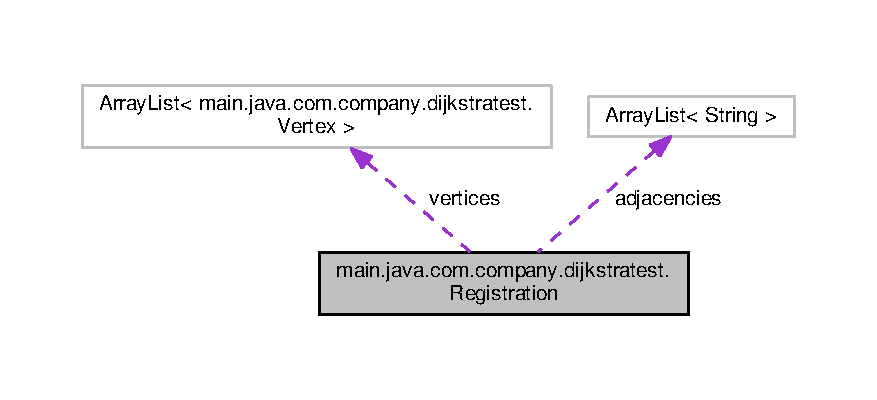
\includegraphics[width=350pt]{classmain_1_1java_1_1com_1_1company_1_1dijkstratest_1_1_registration__coll__graph}
\end{center}
\end{figure}
\subsection*{Public Member Functions}
\begin{DoxyCompactItemize}
\item 
\hyperlink{classmain_1_1java_1_1com_1_1company_1_1dijkstratest_1_1_registration_a0139c70aa03637c99ffbae2142572aba}{Registration} (Array\-List$<$ \hyperlink{classmain_1_1java_1_1com_1_1company_1_1dijkstratest_1_1_vertex}{Vertex} $>$ \hyperlink{classmain_1_1java_1_1com_1_1company_1_1dijkstratest_1_1_registration_aacd4ad524e3c3d2d3e163ba14dc5e5d4}{vertices}, Array\-List$<$ String $>$ \hyperlink{classmain_1_1java_1_1com_1_1company_1_1dijkstratest_1_1_registration_a7a40c90a5de4173de7d70214b1c22700}{adjacencies})
\item 
void \hyperlink{classmain_1_1java_1_1com_1_1company_1_1dijkstratest_1_1_registration_adc93e97fd7f83981bad275bd013f3cc6}{register\-Vertices} (String phones\-File)
\item 
void \hyperlink{classmain_1_1java_1_1com_1_1company_1_1dijkstratest_1_1_registration_a1ce9fa88223cb28f8bd0e1052cadfe95}{register\-Adjacencies} (String adjacencies\-File)
\end{DoxyCompactItemize}
\subsection*{Private Attributes}
\begin{DoxyCompactItemize}
\item 
final Array\-List$<$ String $>$ \hyperlink{classmain_1_1java_1_1com_1_1company_1_1dijkstratest_1_1_registration_a7a40c90a5de4173de7d70214b1c22700}{adjacencies}
\item 
final Array\-List$<$ \hyperlink{classmain_1_1java_1_1com_1_1company_1_1dijkstratest_1_1_vertex}{Vertex} $>$ \hyperlink{classmain_1_1java_1_1com_1_1company_1_1dijkstratest_1_1_registration_aacd4ad524e3c3d2d3e163ba14dc5e5d4}{vertices}
\end{DoxyCompactItemize}


\subsection{Detailed Description}
Read phone information and phones-\/neighborhood relationship info from two files \begin{DoxyAuthor}{Author}
hzhang 
\end{DoxyAuthor}


Definition at line 16 of file Registration.\-java.



\subsection{Constructor \& Destructor Documentation}
\hypertarget{classmain_1_1java_1_1com_1_1company_1_1dijkstratest_1_1_registration_a0139c70aa03637c99ffbae2142572aba}{\index{main\-::java\-::com\-::company\-::dijkstratest\-::\-Registration@{main\-::java\-::com\-::company\-::dijkstratest\-::\-Registration}!Registration@{Registration}}
\index{Registration@{Registration}!main::java::com::company::dijkstratest::Registration@{main\-::java\-::com\-::company\-::dijkstratest\-::\-Registration}}
\subsubsection[{Registration}]{\setlength{\rightskip}{0pt plus 5cm}main.\-java.\-com.\-company.\-dijkstratest.\-Registration.\-Registration (
\begin{DoxyParamCaption}
\item[{Array\-List$<$ {\bf Vertex} $>$}]{vertices, }
\item[{Array\-List$<$ String $>$}]{adjacencies}
\end{DoxyParamCaption}
)}}\label{classmain_1_1java_1_1com_1_1company_1_1dijkstratest_1_1_registration_a0139c70aa03637c99ffbae2142572aba}
Constructor


\begin{DoxyParams}{Parameters}
{\em vertices} & list of all subscribers \\
\hline
{\em adjacencies} & list of connected phone pairs \\
\hline
\end{DoxyParams}


Definition at line 27 of file Registration.\-java.



References main.\-java.\-com.\-company.\-dijkstratest.\-Registration.\-adjacencies, and main.\-java.\-com.\-company.\-dijkstratest.\-Registration.\-vertices.



\subsection{Member Function Documentation}
\hypertarget{classmain_1_1java_1_1com_1_1company_1_1dijkstratest_1_1_registration_a1ce9fa88223cb28f8bd0e1052cadfe95}{\index{main\-::java\-::com\-::company\-::dijkstratest\-::\-Registration@{main\-::java\-::com\-::company\-::dijkstratest\-::\-Registration}!register\-Adjacencies@{register\-Adjacencies}}
\index{register\-Adjacencies@{register\-Adjacencies}!main::java::com::company::dijkstratest::Registration@{main\-::java\-::com\-::company\-::dijkstratest\-::\-Registration}}
\subsubsection[{register\-Adjacencies}]{\setlength{\rightskip}{0pt plus 5cm}void main.\-java.\-com.\-company.\-dijkstratest.\-Registration.\-register\-Adjacencies (
\begin{DoxyParamCaption}
\item[{String}]{adjacencies\-File}
\end{DoxyParamCaption}
)}}\label{classmain_1_1java_1_1com_1_1company_1_1dijkstratest_1_1_registration_a1ce9fa88223cb28f8bd0e1052cadfe95}
Initializing all the phones who call/sms each other. Those \char`\"{}op-\/cp\char`\"{} pairs satisfy with the condition\-: F = 40(S\-M\-S/\-Month) \&\& 240(sec/\-Month) 

Definition at line 64 of file Registration.\-java.

\hypertarget{classmain_1_1java_1_1com_1_1company_1_1dijkstratest_1_1_registration_adc93e97fd7f83981bad275bd013f3cc6}{\index{main\-::java\-::com\-::company\-::dijkstratest\-::\-Registration@{main\-::java\-::com\-::company\-::dijkstratest\-::\-Registration}!register\-Vertices@{register\-Vertices}}
\index{register\-Vertices@{register\-Vertices}!main::java::com::company::dijkstratest::Registration@{main\-::java\-::com\-::company\-::dijkstratest\-::\-Registration}}
\subsubsection[{register\-Vertices}]{\setlength{\rightskip}{0pt plus 5cm}void main.\-java.\-com.\-company.\-dijkstratest.\-Registration.\-register\-Vertices (
\begin{DoxyParamCaption}
\item[{String}]{phones\-File}
\end{DoxyParamCaption}
)}}\label{classmain_1_1java_1_1com_1_1company_1_1dijkstratest_1_1_registration_adc93e97fd7f83981bad275bd013f3cc6}
Register subscribers with its phone numbers 

Definition at line 36 of file Registration.\-java.



\subsection{Member Data Documentation}
\hypertarget{classmain_1_1java_1_1com_1_1company_1_1dijkstratest_1_1_registration_a7a40c90a5de4173de7d70214b1c22700}{\index{main\-::java\-::com\-::company\-::dijkstratest\-::\-Registration@{main\-::java\-::com\-::company\-::dijkstratest\-::\-Registration}!adjacencies@{adjacencies}}
\index{adjacencies@{adjacencies}!main::java::com::company::dijkstratest::Registration@{main\-::java\-::com\-::company\-::dijkstratest\-::\-Registration}}
\subsubsection[{adjacencies}]{\setlength{\rightskip}{0pt plus 5cm}final Array\-List$<$String$>$ main.\-java.\-com.\-company.\-dijkstratest.\-Registration.\-adjacencies\hspace{0.3cm}{\ttfamily [private]}}}\label{classmain_1_1java_1_1com_1_1company_1_1dijkstratest_1_1_registration_a7a40c90a5de4173de7d70214b1c22700}


Definition at line 18 of file Registration.\-java.



Referenced by main.\-java.\-com.\-company.\-dijkstratest.\-Registration.\-Registration().

\hypertarget{classmain_1_1java_1_1com_1_1company_1_1dijkstratest_1_1_registration_aacd4ad524e3c3d2d3e163ba14dc5e5d4}{\index{main\-::java\-::com\-::company\-::dijkstratest\-::\-Registration@{main\-::java\-::com\-::company\-::dijkstratest\-::\-Registration}!vertices@{vertices}}
\index{vertices@{vertices}!main::java::com::company::dijkstratest::Registration@{main\-::java\-::com\-::company\-::dijkstratest\-::\-Registration}}
\subsubsection[{vertices}]{\setlength{\rightskip}{0pt plus 5cm}final Array\-List$<${\bf Vertex}$>$ main.\-java.\-com.\-company.\-dijkstratest.\-Registration.\-vertices\hspace{0.3cm}{\ttfamily [private]}}}\label{classmain_1_1java_1_1com_1_1company_1_1dijkstratest_1_1_registration_aacd4ad524e3c3d2d3e163ba14dc5e5d4}


Definition at line 19 of file Registration.\-java.



Referenced by main.\-java.\-com.\-company.\-dijkstratest.\-Registration.\-Registration().



The documentation for this class was generated from the following file\-:\begin{DoxyCompactItemize}
\item 
src/main/java/com/company/dijkstratest/\hyperlink{_registration_8java}{Registration.\-java}\end{DoxyCompactItemize}

\hypertarget{classmain_1_1java_1_1com_1_1company_1_1dijkstratest_1_1_steps_matrix}{\section{main.\-java.\-com.\-company.\-dijkstratest.\-Steps\-Matrix Class Reference}
\label{classmain_1_1java_1_1com_1_1company_1_1dijkstratest_1_1_steps_matrix}\index{main.\-java.\-com.\-company.\-dijkstratest.\-Steps\-Matrix@{main.\-java.\-com.\-company.\-dijkstratest.\-Steps\-Matrix}}
}


Collaboration diagram for main.\-java.\-com.\-company.\-dijkstratest.\-Steps\-Matrix\-:
\nopagebreak
\begin{figure}[H]
\begin{center}
\leavevmode
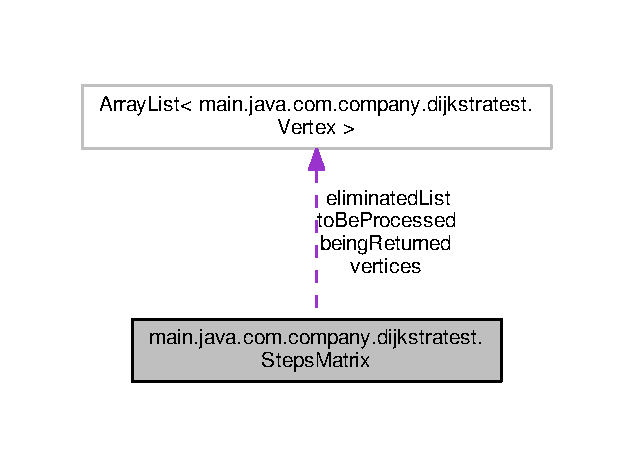
\includegraphics[width=304pt]{classmain_1_1java_1_1com_1_1company_1_1dijkstratest_1_1_steps_matrix__coll__graph}
\end{center}
\end{figure}
\subsection*{Public Member Functions}
\begin{DoxyCompactItemize}
\item 
\hyperlink{classmain_1_1java_1_1com_1_1company_1_1dijkstratest_1_1_steps_matrix_a656c4786dc8adb10dc37018d8c2c1e66}{Steps\-Matrix} (Array\-List$<$ \hyperlink{classmain_1_1java_1_1com_1_1company_1_1dijkstratest_1_1_vertex}{Vertex} $>$ \hyperlink{classmain_1_1java_1_1com_1_1company_1_1dijkstratest_1_1_steps_matrix_a1a3eb1ca85e39b9b704bfe7e26256afb}{vertices}, Array\-List$<$ \hyperlink{classmain_1_1java_1_1com_1_1company_1_1dijkstratest_1_1_vertex}{Vertex} $>$ \hyperlink{classmain_1_1java_1_1com_1_1company_1_1dijkstratest_1_1_steps_matrix_aa51c97e07faba7d835f614554810ab44}{to\-Be\-Processed}, Array\-List$<$ \hyperlink{classmain_1_1java_1_1com_1_1company_1_1dijkstratest_1_1_vertex}{Vertex} $>$ \hyperlink{classmain_1_1java_1_1com_1_1company_1_1dijkstratest_1_1_steps_matrix_af820b561be0222cbf21fd2a6134047b2}{eliminated\-List})
\item 
void \hyperlink{classmain_1_1java_1_1com_1_1company_1_1dijkstratest_1_1_steps_matrix_a25baaea9cd4f24583b9f81b317b88245}{build\-Steps\-Matrix} ()
\item 
void \hyperlink{classmain_1_1java_1_1com_1_1company_1_1dijkstratest_1_1_steps_matrix_a0d41b80e6dd2a43ac0da575866d00a32}{calculate\-Shortest\-Path} (\hyperlink{classmain_1_1java_1_1com_1_1company_1_1dijkstratest_1_1_vertex}{Vertex} source)
\item 
float \hyperlink{classmain_1_1java_1_1com_1_1company_1_1dijkstratest_1_1_steps_matrix_aa0ceb165ab3fe248dace9dce3c9fd1c6}{get\-Centrality} (int diameter)
\item 
void \hyperlink{classmain_1_1java_1_1com_1_1company_1_1dijkstratest_1_1_steps_matrix_a15b14136df6c93f78deff3e498093c5a}{reset} (Array\-List$<$ \hyperlink{classmain_1_1java_1_1com_1_1company_1_1dijkstratest_1_1_vertex}{Vertex} $>$ \hyperlink{classmain_1_1java_1_1com_1_1company_1_1dijkstratest_1_1_steps_matrix_a1a3eb1ca85e39b9b704bfe7e26256afb}{vertices})
\item 
void \hyperlink{classmain_1_1java_1_1com_1_1company_1_1dijkstratest_1_1_steps_matrix_a78a89eed56a05139649e2a34fd6b4fa7}{recovery} (\hyperlink{classmain_1_1java_1_1com_1_1company_1_1dijkstratest_1_1_vertex}{Vertex} source, int diameter)
\end{DoxyCompactItemize}
\subsection*{Private Attributes}
\begin{DoxyCompactItemize}
\item 
Array\-List$<$ \hyperlink{classmain_1_1java_1_1com_1_1company_1_1dijkstratest_1_1_vertex}{Vertex} $>$ \hyperlink{classmain_1_1java_1_1com_1_1company_1_1dijkstratest_1_1_steps_matrix_a1a3eb1ca85e39b9b704bfe7e26256afb}{vertices}
\item 
Array\-List$<$ \hyperlink{classmain_1_1java_1_1com_1_1company_1_1dijkstratest_1_1_vertex}{Vertex} $>$ \hyperlink{classmain_1_1java_1_1com_1_1company_1_1dijkstratest_1_1_steps_matrix_aa51c97e07faba7d835f614554810ab44}{to\-Be\-Processed}
\item 
Array\-List$<$ \hyperlink{classmain_1_1java_1_1com_1_1company_1_1dijkstratest_1_1_vertex}{Vertex} $>$ \hyperlink{classmain_1_1java_1_1com_1_1company_1_1dijkstratest_1_1_steps_matrix_af820b561be0222cbf21fd2a6134047b2}{eliminated\-List}
\item 
Array\-List$<$ \hyperlink{classmain_1_1java_1_1com_1_1company_1_1dijkstratest_1_1_vertex}{Vertex} $>$ \hyperlink{classmain_1_1java_1_1com_1_1company_1_1dijkstratest_1_1_steps_matrix_acb65a2ac68a2b40a4aca6fe2d9276f0d}{being\-Returned} = new Array\-List$<$\hyperlink{classmain_1_1java_1_1com_1_1company_1_1dijkstratest_1_1_vertex}{Vertex}$>$()
\item 
int \hyperlink{classmain_1_1java_1_1com_1_1company_1_1dijkstratest_1_1_steps_matrix_a9f574c424ce414987499434ed7311858}{size}
\end{DoxyCompactItemize}


\subsection{Detailed Description}
\hyperlink{class_dijkstra}{Dijkstra}\-: find the shortest path to vertices \begin{DoxyAuthor}{Author}
hzhang 
\end{DoxyAuthor}


Definition at line 13 of file Steps\-Matrix.\-java.



\subsection{Constructor \& Destructor Documentation}
\hypertarget{classmain_1_1java_1_1com_1_1company_1_1dijkstratest_1_1_steps_matrix_a656c4786dc8adb10dc37018d8c2c1e66}{\index{main\-::java\-::com\-::company\-::dijkstratest\-::\-Steps\-Matrix@{main\-::java\-::com\-::company\-::dijkstratest\-::\-Steps\-Matrix}!Steps\-Matrix@{Steps\-Matrix}}
\index{Steps\-Matrix@{Steps\-Matrix}!main::java::com::company::dijkstratest::StepsMatrix@{main\-::java\-::com\-::company\-::dijkstratest\-::\-Steps\-Matrix}}
\subsubsection[{Steps\-Matrix}]{\setlength{\rightskip}{0pt plus 5cm}main.\-java.\-com.\-company.\-dijkstratest.\-Steps\-Matrix.\-Steps\-Matrix (
\begin{DoxyParamCaption}
\item[{Array\-List$<$ {\bf Vertex} $>$}]{vertices, }
\item[{Array\-List$<$ {\bf Vertex} $>$}]{to\-Be\-Processed, }
\item[{Array\-List$<$ {\bf Vertex} $>$}]{eliminated\-List}
\end{DoxyParamCaption}
)}}\label{classmain_1_1java_1_1com_1_1company_1_1dijkstratest_1_1_steps_matrix_a656c4786dc8adb10dc37018d8c2c1e66}
Constructor 
\begin{DoxyParams}{Parameters}
{\em vertices} & total vertices \\
\hline
{\em to\-Be\-Processed} & community candidates which will be processed \\
\hline
{\em eliminated\-List} & the eliminated vertices \\
\hline
\end{DoxyParams}


Definition at line 27 of file Steps\-Matrix.\-java.



References main.\-java.\-com.\-company.\-dijkstratest.\-Steps\-Matrix.\-eliminated\-List, main.\-java.\-com.\-company.\-dijkstratest.\-Steps\-Matrix.\-size, main.\-java.\-com.\-company.\-dijkstratest.\-Steps\-Matrix.\-to\-Be\-Processed, and main.\-java.\-com.\-company.\-dijkstratest.\-Steps\-Matrix.\-vertices.



\subsection{Member Function Documentation}
\hypertarget{classmain_1_1java_1_1com_1_1company_1_1dijkstratest_1_1_steps_matrix_a25baaea9cd4f24583b9f81b317b88245}{\index{main\-::java\-::com\-::company\-::dijkstratest\-::\-Steps\-Matrix@{main\-::java\-::com\-::company\-::dijkstratest\-::\-Steps\-Matrix}!build\-Steps\-Matrix@{build\-Steps\-Matrix}}
\index{build\-Steps\-Matrix@{build\-Steps\-Matrix}!main::java::com::company::dijkstratest::StepsMatrix@{main\-::java\-::com\-::company\-::dijkstratest\-::\-Steps\-Matrix}}
\subsubsection[{build\-Steps\-Matrix}]{\setlength{\rightskip}{0pt plus 5cm}void main.\-java.\-com.\-company.\-dijkstratest.\-Steps\-Matrix.\-build\-Steps\-Matrix (
\begin{DoxyParamCaption}
{}
\end{DoxyParamCaption}
)}}\label{classmain_1_1java_1_1com_1_1company_1_1dijkstratest_1_1_steps_matrix_a25baaea9cd4f24583b9f81b317b88245}
Build the steps matrix. 

Definition at line 42 of file Steps\-Matrix.\-java.



References main.\-java.\-com.\-company.\-dijkstratest.\-Steps\-Matrix.\-being\-Returned, main.\-java.\-com.\-company.\-dijkstratest.\-Steps\-Matrix.\-calculate\-Shortest\-Path(), main.\-java.\-com.\-company.\-dijkstratest.\-Steps\-Matrix.\-get\-Centrality(), main.\-java.\-com.\-company.\-dijkstratest.\-Steps\-Matrix.\-recovery(), main.\-java.\-com.\-company.\-dijkstratest.\-Steps\-Matrix.\-reset(), main.\-java.\-com.\-company.\-dijkstratest.\-Steps\-Matrix.\-size, main.\-java.\-com.\-company.\-dijkstratest.\-Steps\-Matrix.\-to\-Be\-Processed, and main.\-java.\-com.\-company.\-dijkstratest.\-Steps\-Matrix.\-vertices.



Here is the call graph for this function\-:
\nopagebreak
\begin{figure}[H]
\begin{center}
\leavevmode
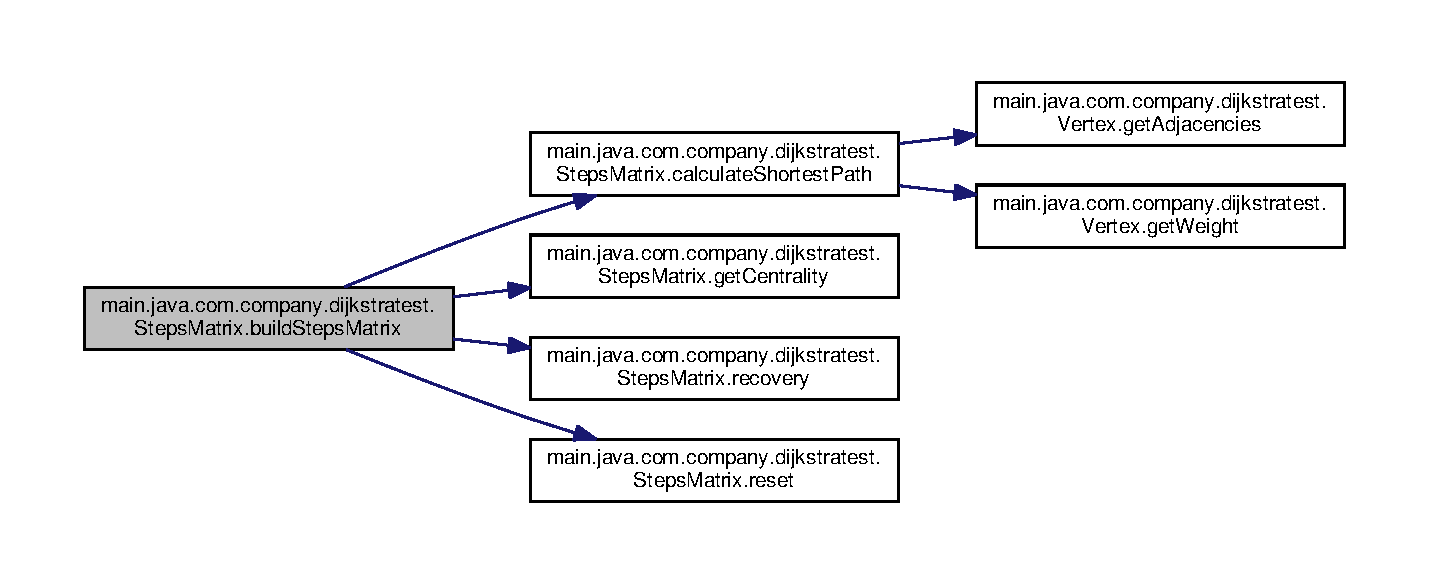
\includegraphics[width=350pt]{classmain_1_1java_1_1com_1_1company_1_1dijkstratest_1_1_steps_matrix_a25baaea9cd4f24583b9f81b317b88245_cgraph}
\end{center}
\end{figure}


\hypertarget{classmain_1_1java_1_1com_1_1company_1_1dijkstratest_1_1_steps_matrix_a0d41b80e6dd2a43ac0da575866d00a32}{\index{main\-::java\-::com\-::company\-::dijkstratest\-::\-Steps\-Matrix@{main\-::java\-::com\-::company\-::dijkstratest\-::\-Steps\-Matrix}!calculate\-Shortest\-Path@{calculate\-Shortest\-Path}}
\index{calculate\-Shortest\-Path@{calculate\-Shortest\-Path}!main::java::com::company::dijkstratest::StepsMatrix@{main\-::java\-::com\-::company\-::dijkstratest\-::\-Steps\-Matrix}}
\subsubsection[{calculate\-Shortest\-Path}]{\setlength{\rightskip}{0pt plus 5cm}void main.\-java.\-com.\-company.\-dijkstratest.\-Steps\-Matrix.\-calculate\-Shortest\-Path (
\begin{DoxyParamCaption}
\item[{{\bf Vertex}}]{source}
\end{DoxyParamCaption}
)}}\label{classmain_1_1java_1_1com_1_1company_1_1dijkstratest_1_1_steps_matrix_a0d41b80e6dd2a43ac0da575866d00a32}
Calculate the shortest path based on D\-I\-J\-K\-S\-T\-R\-A algorithm. 
\begin{DoxyParams}{Parameters}
{\em source} & \\
\hline
\end{DoxyParams}


Definition at line 81 of file Steps\-Matrix.\-java.



References main.\-java.\-com.\-company.\-dijkstratest.\-Vertex.\-get\-Adjacencies(), and main.\-java.\-com.\-company.\-dijkstratest.\-Vertex.\-get\-Weight().



Referenced by main.\-java.\-com.\-company.\-dijkstratest.\-Steps\-Matrix.\-build\-Steps\-Matrix().



Here is the call graph for this function\-:
\nopagebreak
\begin{figure}[H]
\begin{center}
\leavevmode
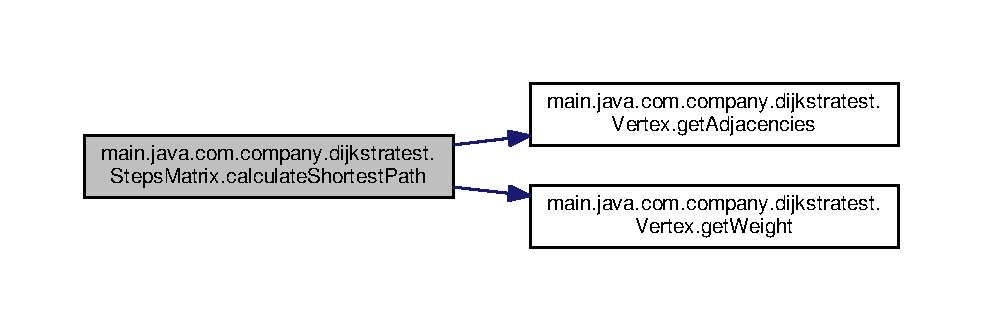
\includegraphics[width=350pt]{classmain_1_1java_1_1com_1_1company_1_1dijkstratest_1_1_steps_matrix_a0d41b80e6dd2a43ac0da575866d00a32_cgraph}
\end{center}
\end{figure}


\hypertarget{classmain_1_1java_1_1com_1_1company_1_1dijkstratest_1_1_steps_matrix_aa0ceb165ab3fe248dace9dce3c9fd1c6}{\index{main\-::java\-::com\-::company\-::dijkstratest\-::\-Steps\-Matrix@{main\-::java\-::com\-::company\-::dijkstratest\-::\-Steps\-Matrix}!get\-Centrality@{get\-Centrality}}
\index{get\-Centrality@{get\-Centrality}!main::java::com::company::dijkstratest::StepsMatrix@{main\-::java\-::com\-::company\-::dijkstratest\-::\-Steps\-Matrix}}
\subsubsection[{get\-Centrality}]{\setlength{\rightskip}{0pt plus 5cm}float main.\-java.\-com.\-company.\-dijkstratest.\-Steps\-Matrix.\-get\-Centrality (
\begin{DoxyParamCaption}
\item[{int}]{diameter}
\end{DoxyParamCaption}
)}}\label{classmain_1_1java_1_1com_1_1company_1_1dijkstratest_1_1_steps_matrix_aa0ceb165ab3fe248dace9dce3c9fd1c6}
Return the centrality with two digits fractions 
\begin{DoxyParams}{Parameters}
{\em diameter} & \\
\hline
\end{DoxyParams}
\begin{DoxyReturn}{Returns}

\end{DoxyReturn}


Definition at line 109 of file Steps\-Matrix.\-java.



Referenced by main.\-java.\-com.\-company.\-dijkstratest.\-Steps\-Matrix.\-build\-Steps\-Matrix().

\hypertarget{classmain_1_1java_1_1com_1_1company_1_1dijkstratest_1_1_steps_matrix_a78a89eed56a05139649e2a34fd6b4fa7}{\index{main\-::java\-::com\-::company\-::dijkstratest\-::\-Steps\-Matrix@{main\-::java\-::com\-::company\-::dijkstratest\-::\-Steps\-Matrix}!recovery@{recovery}}
\index{recovery@{recovery}!main::java::com::company::dijkstratest::StepsMatrix@{main\-::java\-::com\-::company\-::dijkstratest\-::\-Steps\-Matrix}}
\subsubsection[{recovery}]{\setlength{\rightskip}{0pt plus 5cm}void main.\-java.\-com.\-company.\-dijkstratest.\-Steps\-Matrix.\-recovery (
\begin{DoxyParamCaption}
\item[{{\bf Vertex}}]{source, }
\item[{int}]{diameter}
\end{DoxyParamCaption}
)}}\label{classmain_1_1java_1_1com_1_1company_1_1dijkstratest_1_1_steps_matrix_a78a89eed56a05139649e2a34fd6b4fa7}
put the vertices whose diameter $>$ 10 back to the original vertices 
\begin{DoxyParams}{Parameters}
{\em source} & \\
\hline
{\em diameter} & \\
\hline
\end{DoxyParams}


Definition at line 132 of file Steps\-Matrix.\-java.



References main.\-java.\-com.\-company.\-dijkstratest.\-Steps\-Matrix.\-to\-Be\-Processed.



Referenced by main.\-java.\-com.\-company.\-dijkstratest.\-Steps\-Matrix.\-build\-Steps\-Matrix().

\hypertarget{classmain_1_1java_1_1com_1_1company_1_1dijkstratest_1_1_steps_matrix_a15b14136df6c93f78deff3e498093c5a}{\index{main\-::java\-::com\-::company\-::dijkstratest\-::\-Steps\-Matrix@{main\-::java\-::com\-::company\-::dijkstratest\-::\-Steps\-Matrix}!reset@{reset}}
\index{reset@{reset}!main::java::com::company::dijkstratest::StepsMatrix@{main\-::java\-::com\-::company\-::dijkstratest\-::\-Steps\-Matrix}}
\subsubsection[{reset}]{\setlength{\rightskip}{0pt plus 5cm}void main.\-java.\-com.\-company.\-dijkstratest.\-Steps\-Matrix.\-reset (
\begin{DoxyParamCaption}
\item[{Array\-List$<$ {\bf Vertex} $>$}]{vertices}
\end{DoxyParamCaption}
)}}\label{classmain_1_1java_1_1com_1_1company_1_1dijkstratest_1_1_steps_matrix_a15b14136df6c93f78deff3e498093c5a}
Reset the minimum value to 0 
\begin{DoxyParams}{Parameters}
{\em vertices} & \\
\hline
\end{DoxyParams}


Definition at line 119 of file Steps\-Matrix.\-java.



Referenced by main.\-java.\-com.\-company.\-dijkstratest.\-Steps\-Matrix.\-build\-Steps\-Matrix().



\subsection{Member Data Documentation}
\hypertarget{classmain_1_1java_1_1com_1_1company_1_1dijkstratest_1_1_steps_matrix_acb65a2ac68a2b40a4aca6fe2d9276f0d}{\index{main\-::java\-::com\-::company\-::dijkstratest\-::\-Steps\-Matrix@{main\-::java\-::com\-::company\-::dijkstratest\-::\-Steps\-Matrix}!being\-Returned@{being\-Returned}}
\index{being\-Returned@{being\-Returned}!main::java::com::company::dijkstratest::StepsMatrix@{main\-::java\-::com\-::company\-::dijkstratest\-::\-Steps\-Matrix}}
\subsubsection[{being\-Returned}]{\setlength{\rightskip}{0pt plus 5cm}Array\-List$<${\bf Vertex}$>$ main.\-java.\-com.\-company.\-dijkstratest.\-Steps\-Matrix.\-being\-Returned = new Array\-List$<${\bf Vertex}$>$()\hspace{0.3cm}{\ttfamily [private]}}}\label{classmain_1_1java_1_1com_1_1company_1_1dijkstratest_1_1_steps_matrix_acb65a2ac68a2b40a4aca6fe2d9276f0d}


Definition at line 18 of file Steps\-Matrix.\-java.



Referenced by main.\-java.\-com.\-company.\-dijkstratest.\-Steps\-Matrix.\-build\-Steps\-Matrix().

\hypertarget{classmain_1_1java_1_1com_1_1company_1_1dijkstratest_1_1_steps_matrix_af820b561be0222cbf21fd2a6134047b2}{\index{main\-::java\-::com\-::company\-::dijkstratest\-::\-Steps\-Matrix@{main\-::java\-::com\-::company\-::dijkstratest\-::\-Steps\-Matrix}!eliminated\-List@{eliminated\-List}}
\index{eliminated\-List@{eliminated\-List}!main::java::com::company::dijkstratest::StepsMatrix@{main\-::java\-::com\-::company\-::dijkstratest\-::\-Steps\-Matrix}}
\subsubsection[{eliminated\-List}]{\setlength{\rightskip}{0pt plus 5cm}Array\-List$<${\bf Vertex}$>$ main.\-java.\-com.\-company.\-dijkstratest.\-Steps\-Matrix.\-eliminated\-List\hspace{0.3cm}{\ttfamily [private]}}}\label{classmain_1_1java_1_1com_1_1company_1_1dijkstratest_1_1_steps_matrix_af820b561be0222cbf21fd2a6134047b2}


Definition at line 17 of file Steps\-Matrix.\-java.



Referenced by main.\-java.\-com.\-company.\-dijkstratest.\-Steps\-Matrix.\-Steps\-Matrix().

\hypertarget{classmain_1_1java_1_1com_1_1company_1_1dijkstratest_1_1_steps_matrix_a9f574c424ce414987499434ed7311858}{\index{main\-::java\-::com\-::company\-::dijkstratest\-::\-Steps\-Matrix@{main\-::java\-::com\-::company\-::dijkstratest\-::\-Steps\-Matrix}!size@{size}}
\index{size@{size}!main::java::com::company::dijkstratest::StepsMatrix@{main\-::java\-::com\-::company\-::dijkstratest\-::\-Steps\-Matrix}}
\subsubsection[{size}]{\setlength{\rightskip}{0pt plus 5cm}int main.\-java.\-com.\-company.\-dijkstratest.\-Steps\-Matrix.\-size\hspace{0.3cm}{\ttfamily [private]}}}\label{classmain_1_1java_1_1com_1_1company_1_1dijkstratest_1_1_steps_matrix_a9f574c424ce414987499434ed7311858}


Definition at line 19 of file Steps\-Matrix.\-java.



Referenced by main.\-java.\-com.\-company.\-dijkstratest.\-Steps\-Matrix.\-build\-Steps\-Matrix(), and main.\-java.\-com.\-company.\-dijkstratest.\-Steps\-Matrix.\-Steps\-Matrix().

\hypertarget{classmain_1_1java_1_1com_1_1company_1_1dijkstratest_1_1_steps_matrix_aa51c97e07faba7d835f614554810ab44}{\index{main\-::java\-::com\-::company\-::dijkstratest\-::\-Steps\-Matrix@{main\-::java\-::com\-::company\-::dijkstratest\-::\-Steps\-Matrix}!to\-Be\-Processed@{to\-Be\-Processed}}
\index{to\-Be\-Processed@{to\-Be\-Processed}!main::java::com::company::dijkstratest::StepsMatrix@{main\-::java\-::com\-::company\-::dijkstratest\-::\-Steps\-Matrix}}
\subsubsection[{to\-Be\-Processed}]{\setlength{\rightskip}{0pt plus 5cm}Array\-List$<${\bf Vertex}$>$ main.\-java.\-com.\-company.\-dijkstratest.\-Steps\-Matrix.\-to\-Be\-Processed\hspace{0.3cm}{\ttfamily [private]}}}\label{classmain_1_1java_1_1com_1_1company_1_1dijkstratest_1_1_steps_matrix_aa51c97e07faba7d835f614554810ab44}


Definition at line 16 of file Steps\-Matrix.\-java.



Referenced by main.\-java.\-com.\-company.\-dijkstratest.\-Steps\-Matrix.\-build\-Steps\-Matrix(), main.\-java.\-com.\-company.\-dijkstratest.\-Steps\-Matrix.\-recovery(), and main.\-java.\-com.\-company.\-dijkstratest.\-Steps\-Matrix.\-Steps\-Matrix().

\hypertarget{classmain_1_1java_1_1com_1_1company_1_1dijkstratest_1_1_steps_matrix_a1a3eb1ca85e39b9b704bfe7e26256afb}{\index{main\-::java\-::com\-::company\-::dijkstratest\-::\-Steps\-Matrix@{main\-::java\-::com\-::company\-::dijkstratest\-::\-Steps\-Matrix}!vertices@{vertices}}
\index{vertices@{vertices}!main::java::com::company::dijkstratest::StepsMatrix@{main\-::java\-::com\-::company\-::dijkstratest\-::\-Steps\-Matrix}}
\subsubsection[{vertices}]{\setlength{\rightskip}{0pt plus 5cm}Array\-List$<${\bf Vertex}$>$ main.\-java.\-com.\-company.\-dijkstratest.\-Steps\-Matrix.\-vertices\hspace{0.3cm}{\ttfamily [private]}}}\label{classmain_1_1java_1_1com_1_1company_1_1dijkstratest_1_1_steps_matrix_a1a3eb1ca85e39b9b704bfe7e26256afb}


Definition at line 15 of file Steps\-Matrix.\-java.



Referenced by main.\-java.\-com.\-company.\-dijkstratest.\-Steps\-Matrix.\-build\-Steps\-Matrix(), and main.\-java.\-com.\-company.\-dijkstratest.\-Steps\-Matrix.\-Steps\-Matrix().



The documentation for this class was generated from the following file\-:\begin{DoxyCompactItemize}
\item 
src/main/java/com/company/dijkstratest/\hyperlink{_steps_matrix_8java}{Steps\-Matrix.\-java}\end{DoxyCompactItemize}

\hypertarget{classmain_1_1java_1_1com_1_1company_1_1dijkstratest_1_1_vertex}{\section{main.\-java.\-com.\-company.\-dijkstratest.\-Vertex Class Reference}
\label{classmain_1_1java_1_1com_1_1company_1_1dijkstratest_1_1_vertex}\index{main.\-java.\-com.\-company.\-dijkstratest.\-Vertex@{main.\-java.\-com.\-company.\-dijkstratest.\-Vertex}}
}


Inheritance diagram for main.\-java.\-com.\-company.\-dijkstratest.\-Vertex\-:
\nopagebreak
\begin{figure}[H]
\begin{center}
\leavevmode
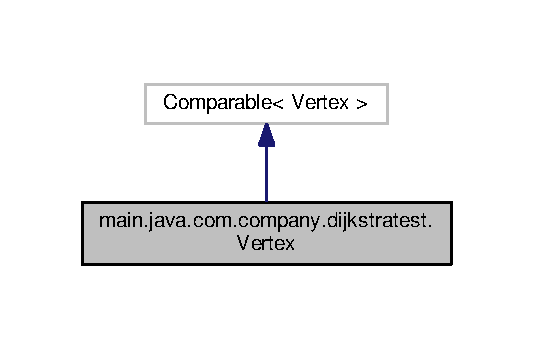
\includegraphics[width=256pt]{classmain_1_1java_1_1com_1_1company_1_1dijkstratest_1_1_vertex__inherit__graph}
\end{center}
\end{figure}


Collaboration diagram for main.\-java.\-com.\-company.\-dijkstratest.\-Vertex\-:
\nopagebreak
\begin{figure}[H]
\begin{center}
\leavevmode
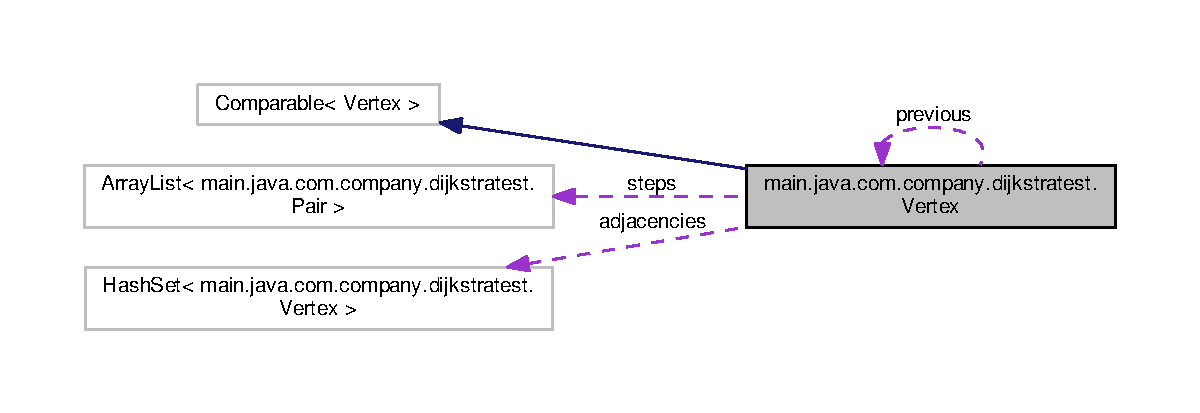
\includegraphics[width=350pt]{classmain_1_1java_1_1com_1_1company_1_1dijkstratest_1_1_vertex__coll__graph}
\end{center}
\end{figure}
\subsection*{Public Member Functions}
\begin{DoxyCompactItemize}
\item 
\hyperlink{classmain_1_1java_1_1com_1_1company_1_1dijkstratest_1_1_vertex_a5c4df011dc24230cf67918f0d1c6b8f9}{Vertex} (String \hyperlink{classmain_1_1java_1_1com_1_1company_1_1dijkstratest_1_1_vertex_a2d3af47cee45105338487ebabe5d41af}{name})
\item 
int \hyperlink{classmain_1_1java_1_1com_1_1company_1_1dijkstratest_1_1_vertex_a37e1d362f47485e54f2e0a9cf56ac8c3}{get\-Weight} ()
\item 
void \hyperlink{classmain_1_1java_1_1com_1_1company_1_1dijkstratest_1_1_vertex_afe351de304209254ba6efdfdff362a27}{set\-Min\-Distance} (int distance)
\item 
int \hyperlink{classmain_1_1java_1_1com_1_1company_1_1dijkstratest_1_1_vertex_a0afd4e2eb4689ac8a4682b3c0f6e32d2}{get\-Min\-Distance} ()
\item 
void \hyperlink{classmain_1_1java_1_1com_1_1company_1_1dijkstratest_1_1_vertex_aec5f28d756beeb653fa52e733c2db139}{set\-Previous} (\hyperlink{classmain_1_1java_1_1com_1_1company_1_1dijkstratest_1_1_vertex}{Vertex} vertex)
\item 
\hyperlink{classmain_1_1java_1_1com_1_1company_1_1dijkstratest_1_1_vertex}{Vertex} \hyperlink{classmain_1_1java_1_1com_1_1company_1_1dijkstratest_1_1_vertex_a925585cbe8eb8ee5bf74b0cb58d388df}{get\-Previous} ()
\item 
void \hyperlink{classmain_1_1java_1_1com_1_1company_1_1dijkstratest_1_1_vertex_aec87153fc8c4f42b11c97c9566c9bfd9}{set\-Adjacencies} (Vertex...\-vertex\-List)
\item 
Hash\-Set$<$ \hyperlink{classmain_1_1java_1_1com_1_1company_1_1dijkstratest_1_1_vertex}{Vertex} $>$ \hyperlink{classmain_1_1java_1_1com_1_1company_1_1dijkstratest_1_1_vertex_ad4896ef0f829054d9a765436cdda7804}{get\-Adjacencies} ()
\item 
void \hyperlink{classmain_1_1java_1_1com_1_1company_1_1dijkstratest_1_1_vertex_ab66f86a13171527e0c762e90eef3dc5e}{set\-Steps} (\hyperlink{classmain_1_1java_1_1com_1_1company_1_1dijkstratest_1_1_vertex}{Vertex} v, int integer)
\item 
Array\-List$<$ \hyperlink{classmain_1_1java_1_1com_1_1company_1_1dijkstratest_1_1_pair}{Pair} $>$ \hyperlink{classmain_1_1java_1_1com_1_1company_1_1dijkstratest_1_1_vertex_aac9933bc854f3b3a427c7467824e29de}{get\-Steps} ()
\item 
String \hyperlink{classmain_1_1java_1_1com_1_1company_1_1dijkstratest_1_1_vertex_a05c58848e7052edb8f08e827a84fcca2}{get\-Name} ()
\item 
void \hyperlink{classmain_1_1java_1_1com_1_1company_1_1dijkstratest_1_1_vertex_aa1ee193d9f7d429f80d3fb2f1f2df58e}{set\-Diameter} (int \hyperlink{classmain_1_1java_1_1com_1_1company_1_1dijkstratest_1_1_vertex_af5f0b296f64910fb629a69b8e39b6498}{diameter})
\item 
int \hyperlink{classmain_1_1java_1_1com_1_1company_1_1dijkstratest_1_1_vertex_a7db864a45fcb444f523cdff89a68479a}{get\-Diameter} ()
\item 
String \hyperlink{classmain_1_1java_1_1com_1_1company_1_1dijkstratest_1_1_vertex_a1c40f05bb5ba581ad9c48b7a26027310}{to\-String} ()
\item 
int \hyperlink{classmain_1_1java_1_1com_1_1company_1_1dijkstratest_1_1_vertex_a5fc177277ea1d740a9bfcc71d58fe439}{compare\-To} (\hyperlink{classmain_1_1java_1_1com_1_1company_1_1dijkstratest_1_1_vertex}{Vertex} other)
\item 
void \hyperlink{classmain_1_1java_1_1com_1_1company_1_1dijkstratest_1_1_vertex_a79d03d4b51e85227fd64ee15a54895bb}{remove\-Steps} (\hyperlink{classmain_1_1java_1_1com_1_1company_1_1dijkstratest_1_1_vertex}{Vertex} v)
\end{DoxyCompactItemize}
\subsection*{Private Attributes}
\begin{DoxyCompactItemize}
\item 
final int \hyperlink{classmain_1_1java_1_1com_1_1company_1_1dijkstratest_1_1_vertex_a17e38182d49640463ff2a93a55dd12d8}{weight} = 1
\item 
int \hyperlink{classmain_1_1java_1_1com_1_1company_1_1dijkstratest_1_1_vertex_a4ea46fdc17ccba35d2a35e4b70bff997}{min\-Distance} = Integer.\-M\-A\-X\-\_\-\-V\-A\-L\-U\-E
\item 
\hyperlink{classmain_1_1java_1_1com_1_1company_1_1dijkstratest_1_1_vertex}{Vertex} \hyperlink{classmain_1_1java_1_1com_1_1company_1_1dijkstratest_1_1_vertex_a748206c2f117a19e74469881e71b2415}{previous}
\item 
Hash\-Set$<$ \hyperlink{classmain_1_1java_1_1com_1_1company_1_1dijkstratest_1_1_vertex}{Vertex} $>$ \hyperlink{classmain_1_1java_1_1com_1_1company_1_1dijkstratest_1_1_vertex_acb5df443c451a3c4f11b48b4fd5a7c46}{adjacencies} = new Hash\-Set$<$\hyperlink{classmain_1_1java_1_1com_1_1company_1_1dijkstratest_1_1_vertex}{Vertex}$>$()
\item 
Array\-List$<$ \hyperlink{classmain_1_1java_1_1com_1_1company_1_1dijkstratest_1_1_pair}{Pair} $>$ \hyperlink{classmain_1_1java_1_1com_1_1company_1_1dijkstratest_1_1_vertex_a21bd658cd178bffda298570f221cdfce}{steps} = new Array\-List$<$\hyperlink{classmain_1_1java_1_1com_1_1company_1_1dijkstratest_1_1_pair}{Pair}$>$()
\item 
final String \hyperlink{classmain_1_1java_1_1com_1_1company_1_1dijkstratest_1_1_vertex_a2d3af47cee45105338487ebabe5d41af}{name}
\item 
int \hyperlink{classmain_1_1java_1_1com_1_1company_1_1dijkstratest_1_1_vertex_af5f0b296f64910fb629a69b8e39b6498}{diameter} = 0
\end{DoxyCompactItemize}


\subsection{Detailed Description}
\hyperlink{classmain_1_1java_1_1com_1_1company_1_1dijkstratest_1_1_vertex}{Vertex} Information \begin{DoxyAuthor}{Author}
hzhang 
\end{DoxyAuthor}


Definition at line 11 of file Vertex.\-java.



\subsection{Constructor \& Destructor Documentation}
\hypertarget{classmain_1_1java_1_1com_1_1company_1_1dijkstratest_1_1_vertex_a5c4df011dc24230cf67918f0d1c6b8f9}{\index{main\-::java\-::com\-::company\-::dijkstratest\-::\-Vertex@{main\-::java\-::com\-::company\-::dijkstratest\-::\-Vertex}!Vertex@{Vertex}}
\index{Vertex@{Vertex}!main::java::com::company::dijkstratest::Vertex@{main\-::java\-::com\-::company\-::dijkstratest\-::\-Vertex}}
\subsubsection[{Vertex}]{\setlength{\rightskip}{0pt plus 5cm}main.\-java.\-com.\-company.\-dijkstratest.\-Vertex.\-Vertex (
\begin{DoxyParamCaption}
\item[{String}]{name}
\end{DoxyParamCaption}
)}}\label{classmain_1_1java_1_1com_1_1company_1_1dijkstratest_1_1_vertex_a5c4df011dc24230cf67918f0d1c6b8f9}
Constructor Initial vertex name and default weight


\begin{DoxyParams}{Parameters}
{\em name} & vertex name \\
\hline
\end{DoxyParams}


Definition at line 19 of file Vertex.\-java.



References main.\-java.\-com.\-company.\-dijkstratest.\-Vertex.\-name.



\subsection{Member Function Documentation}
\hypertarget{classmain_1_1java_1_1com_1_1company_1_1dijkstratest_1_1_vertex_a5fc177277ea1d740a9bfcc71d58fe439}{\index{main\-::java\-::com\-::company\-::dijkstratest\-::\-Vertex@{main\-::java\-::com\-::company\-::dijkstratest\-::\-Vertex}!compare\-To@{compare\-To}}
\index{compare\-To@{compare\-To}!main::java::com::company::dijkstratest::Vertex@{main\-::java\-::com\-::company\-::dijkstratest\-::\-Vertex}}
\subsubsection[{compare\-To}]{\setlength{\rightskip}{0pt plus 5cm}int main.\-java.\-com.\-company.\-dijkstratest.\-Vertex.\-compare\-To (
\begin{DoxyParamCaption}
\item[{{\bf Vertex}}]{other}
\end{DoxyParamCaption}
)}}\label{classmain_1_1java_1_1com_1_1company_1_1dijkstratest_1_1_vertex_a5fc177277ea1d740a9bfcc71d58fe439}


Definition at line 70 of file Vertex.\-java.



References main.\-java.\-com.\-company.\-dijkstratest.\-Vertex.\-get\-Name().



Here is the call graph for this function\-:
\nopagebreak
\begin{figure}[H]
\begin{center}
\leavevmode
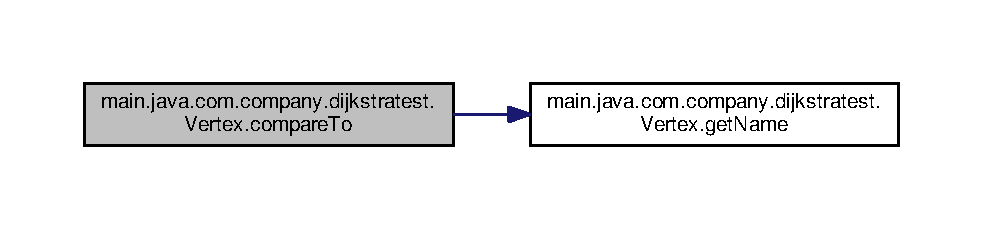
\includegraphics[width=350pt]{classmain_1_1java_1_1com_1_1company_1_1dijkstratest_1_1_vertex_a5fc177277ea1d740a9bfcc71d58fe439_cgraph}
\end{center}
\end{figure}


\hypertarget{classmain_1_1java_1_1com_1_1company_1_1dijkstratest_1_1_vertex_ad4896ef0f829054d9a765436cdda7804}{\index{main\-::java\-::com\-::company\-::dijkstratest\-::\-Vertex@{main\-::java\-::com\-::company\-::dijkstratest\-::\-Vertex}!get\-Adjacencies@{get\-Adjacencies}}
\index{get\-Adjacencies@{get\-Adjacencies}!main::java::com::company::dijkstratest::Vertex@{main\-::java\-::com\-::company\-::dijkstratest\-::\-Vertex}}
\subsubsection[{get\-Adjacencies}]{\setlength{\rightskip}{0pt plus 5cm}Hash\-Set$<${\bf Vertex}$>$ main.\-java.\-com.\-company.\-dijkstratest.\-Vertex.\-get\-Adjacencies (
\begin{DoxyParamCaption}
{}
\end{DoxyParamCaption}
)}}\label{classmain_1_1java_1_1com_1_1company_1_1dijkstratest_1_1_vertex_ad4896ef0f829054d9a765436cdda7804}


Definition at line 44 of file Vertex.\-java.



References main.\-java.\-com.\-company.\-dijkstratest.\-Vertex.\-adjacencies.



Referenced by main.\-java.\-com.\-company.\-dijkstratest.\-Steps\-Matrix.\-calculate\-Shortest\-Path().

\hypertarget{classmain_1_1java_1_1com_1_1company_1_1dijkstratest_1_1_vertex_a7db864a45fcb444f523cdff89a68479a}{\index{main\-::java\-::com\-::company\-::dijkstratest\-::\-Vertex@{main\-::java\-::com\-::company\-::dijkstratest\-::\-Vertex}!get\-Diameter@{get\-Diameter}}
\index{get\-Diameter@{get\-Diameter}!main::java::com::company::dijkstratest::Vertex@{main\-::java\-::com\-::company\-::dijkstratest\-::\-Vertex}}
\subsubsection[{get\-Diameter}]{\setlength{\rightskip}{0pt plus 5cm}int main.\-java.\-com.\-company.\-dijkstratest.\-Vertex.\-get\-Diameter (
\begin{DoxyParamCaption}
{}
\end{DoxyParamCaption}
)}}\label{classmain_1_1java_1_1com_1_1company_1_1dijkstratest_1_1_vertex_a7db864a45fcb444f523cdff89a68479a}


Definition at line 64 of file Vertex.\-java.

\hypertarget{classmain_1_1java_1_1com_1_1company_1_1dijkstratest_1_1_vertex_a0afd4e2eb4689ac8a4682b3c0f6e32d2}{\index{main\-::java\-::com\-::company\-::dijkstratest\-::\-Vertex@{main\-::java\-::com\-::company\-::dijkstratest\-::\-Vertex}!get\-Min\-Distance@{get\-Min\-Distance}}
\index{get\-Min\-Distance@{get\-Min\-Distance}!main::java::com::company::dijkstratest::Vertex@{main\-::java\-::com\-::company\-::dijkstratest\-::\-Vertex}}
\subsubsection[{get\-Min\-Distance}]{\setlength{\rightskip}{0pt plus 5cm}int main.\-java.\-com.\-company.\-dijkstratest.\-Vertex.\-get\-Min\-Distance (
\begin{DoxyParamCaption}
{}
\end{DoxyParamCaption}
)}}\label{classmain_1_1java_1_1com_1_1company_1_1dijkstratest_1_1_vertex_a0afd4e2eb4689ac8a4682b3c0f6e32d2}


Definition at line 33 of file Vertex.\-java.



References main.\-java.\-com.\-company.\-dijkstratest.\-Vertex.\-min\-Distance.

\hypertarget{classmain_1_1java_1_1com_1_1company_1_1dijkstratest_1_1_vertex_a05c58848e7052edb8f08e827a84fcca2}{\index{main\-::java\-::com\-::company\-::dijkstratest\-::\-Vertex@{main\-::java\-::com\-::company\-::dijkstratest\-::\-Vertex}!get\-Name@{get\-Name}}
\index{get\-Name@{get\-Name}!main::java::com::company::dijkstratest::Vertex@{main\-::java\-::com\-::company\-::dijkstratest\-::\-Vertex}}
\subsubsection[{get\-Name}]{\setlength{\rightskip}{0pt plus 5cm}String main.\-java.\-com.\-company.\-dijkstratest.\-Vertex.\-get\-Name (
\begin{DoxyParamCaption}
{}
\end{DoxyParamCaption}
)}}\label{classmain_1_1java_1_1com_1_1company_1_1dijkstratest_1_1_vertex_a05c58848e7052edb8f08e827a84fcca2}


Definition at line 57 of file Vertex.\-java.



References main.\-java.\-com.\-company.\-dijkstratest.\-Vertex.\-name.



Referenced by main.\-java.\-com.\-company.\-dijkstratest.\-Vertex.\-compare\-To(), and main.\-java.\-com.\-company.\-dijkstratest.\-Vertex.\-remove\-Steps().

\hypertarget{classmain_1_1java_1_1com_1_1company_1_1dijkstratest_1_1_vertex_a925585cbe8eb8ee5bf74b0cb58d388df}{\index{main\-::java\-::com\-::company\-::dijkstratest\-::\-Vertex@{main\-::java\-::com\-::company\-::dijkstratest\-::\-Vertex}!get\-Previous@{get\-Previous}}
\index{get\-Previous@{get\-Previous}!main::java::com::company::dijkstratest::Vertex@{main\-::java\-::com\-::company\-::dijkstratest\-::\-Vertex}}
\subsubsection[{get\-Previous}]{\setlength{\rightskip}{0pt plus 5cm}{\bf Vertex} main.\-java.\-com.\-company.\-dijkstratest.\-Vertex.\-get\-Previous (
\begin{DoxyParamCaption}
{}
\end{DoxyParamCaption}
)}}\label{classmain_1_1java_1_1com_1_1company_1_1dijkstratest_1_1_vertex_a925585cbe8eb8ee5bf74b0cb58d388df}


Definition at line 40 of file Vertex.\-java.



References main.\-java.\-com.\-company.\-dijkstratest.\-Vertex.\-previous.

\hypertarget{classmain_1_1java_1_1com_1_1company_1_1dijkstratest_1_1_vertex_aac9933bc854f3b3a427c7467824e29de}{\index{main\-::java\-::com\-::company\-::dijkstratest\-::\-Vertex@{main\-::java\-::com\-::company\-::dijkstratest\-::\-Vertex}!get\-Steps@{get\-Steps}}
\index{get\-Steps@{get\-Steps}!main::java::com::company::dijkstratest::Vertex@{main\-::java\-::com\-::company\-::dijkstratest\-::\-Vertex}}
\subsubsection[{get\-Steps}]{\setlength{\rightskip}{0pt plus 5cm}Array\-List$<${\bf Pair}$>$ main.\-java.\-com.\-company.\-dijkstratest.\-Vertex.\-get\-Steps (
\begin{DoxyParamCaption}
{}
\end{DoxyParamCaption}
)}}\label{classmain_1_1java_1_1com_1_1company_1_1dijkstratest_1_1_vertex_aac9933bc854f3b3a427c7467824e29de}


Definition at line 51 of file Vertex.\-java.



References main.\-java.\-com.\-company.\-dijkstratest.\-Vertex.\-steps.

\hypertarget{classmain_1_1java_1_1com_1_1company_1_1dijkstratest_1_1_vertex_a37e1d362f47485e54f2e0a9cf56ac8c3}{\index{main\-::java\-::com\-::company\-::dijkstratest\-::\-Vertex@{main\-::java\-::com\-::company\-::dijkstratest\-::\-Vertex}!get\-Weight@{get\-Weight}}
\index{get\-Weight@{get\-Weight}!main::java::com::company::dijkstratest::Vertex@{main\-::java\-::com\-::company\-::dijkstratest\-::\-Vertex}}
\subsubsection[{get\-Weight}]{\setlength{\rightskip}{0pt plus 5cm}int main.\-java.\-com.\-company.\-dijkstratest.\-Vertex.\-get\-Weight (
\begin{DoxyParamCaption}
{}
\end{DoxyParamCaption}
)}}\label{classmain_1_1java_1_1com_1_1company_1_1dijkstratest_1_1_vertex_a37e1d362f47485e54f2e0a9cf56ac8c3}


Definition at line 26 of file Vertex.\-java.



References main.\-java.\-com.\-company.\-dijkstratest.\-Vertex.\-weight.



Referenced by main.\-java.\-com.\-company.\-dijkstratest.\-Steps\-Matrix.\-calculate\-Shortest\-Path().

\hypertarget{classmain_1_1java_1_1com_1_1company_1_1dijkstratest_1_1_vertex_a79d03d4b51e85227fd64ee15a54895bb}{\index{main\-::java\-::com\-::company\-::dijkstratest\-::\-Vertex@{main\-::java\-::com\-::company\-::dijkstratest\-::\-Vertex}!remove\-Steps@{remove\-Steps}}
\index{remove\-Steps@{remove\-Steps}!main::java::com::company::dijkstratest::Vertex@{main\-::java\-::com\-::company\-::dijkstratest\-::\-Vertex}}
\subsubsection[{remove\-Steps}]{\setlength{\rightskip}{0pt plus 5cm}void main.\-java.\-com.\-company.\-dijkstratest.\-Vertex.\-remove\-Steps (
\begin{DoxyParamCaption}
\item[{{\bf Vertex}}]{v}
\end{DoxyParamCaption}
)}}\label{classmain_1_1java_1_1com_1_1company_1_1dijkstratest_1_1_vertex_a79d03d4b51e85227fd64ee15a54895bb}


Definition at line 72 of file Vertex.\-java.



References main.\-java.\-com.\-company.\-dijkstratest.\-Vertex.\-get\-Name(), and main.\-java.\-com.\-company.\-dijkstratest.\-Vertex.\-steps.



Here is the call graph for this function\-:
\nopagebreak
\begin{figure}[H]
\begin{center}
\leavevmode
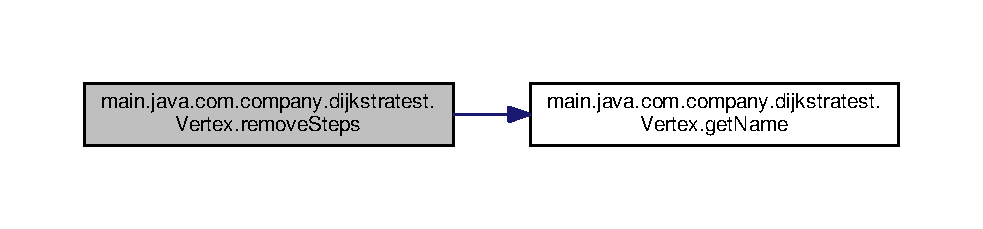
\includegraphics[width=350pt]{classmain_1_1java_1_1com_1_1company_1_1dijkstratest_1_1_vertex_a79d03d4b51e85227fd64ee15a54895bb_cgraph}
\end{center}
\end{figure}


\hypertarget{classmain_1_1java_1_1com_1_1company_1_1dijkstratest_1_1_vertex_aec87153fc8c4f42b11c97c9566c9bfd9}{\index{main\-::java\-::com\-::company\-::dijkstratest\-::\-Vertex@{main\-::java\-::com\-::company\-::dijkstratest\-::\-Vertex}!set\-Adjacencies@{set\-Adjacencies}}
\index{set\-Adjacencies@{set\-Adjacencies}!main::java::com::company::dijkstratest::Vertex@{main\-::java\-::com\-::company\-::dijkstratest\-::\-Vertex}}
\subsubsection[{set\-Adjacencies}]{\setlength{\rightskip}{0pt plus 5cm}void main.\-java.\-com.\-company.\-dijkstratest.\-Vertex.\-set\-Adjacencies (
\begin{DoxyParamCaption}
\item[{Vertex...}]{vertex\-List}
\end{DoxyParamCaption}
)}}\label{classmain_1_1java_1_1com_1_1company_1_1dijkstratest_1_1_vertex_aec87153fc8c4f42b11c97c9566c9bfd9}


Definition at line 43 of file Vertex.\-java.

\hypertarget{classmain_1_1java_1_1com_1_1company_1_1dijkstratest_1_1_vertex_aa1ee193d9f7d429f80d3fb2f1f2df58e}{\index{main\-::java\-::com\-::company\-::dijkstratest\-::\-Vertex@{main\-::java\-::com\-::company\-::dijkstratest\-::\-Vertex}!set\-Diameter@{set\-Diameter}}
\index{set\-Diameter@{set\-Diameter}!main::java::com::company::dijkstratest::Vertex@{main\-::java\-::com\-::company\-::dijkstratest\-::\-Vertex}}
\subsubsection[{set\-Diameter}]{\setlength{\rightskip}{0pt plus 5cm}void main.\-java.\-com.\-company.\-dijkstratest.\-Vertex.\-set\-Diameter (
\begin{DoxyParamCaption}
\item[{int}]{diameter}
\end{DoxyParamCaption}
)}}\label{classmain_1_1java_1_1com_1_1company_1_1dijkstratest_1_1_vertex_aa1ee193d9f7d429f80d3fb2f1f2df58e}


Definition at line 63 of file Vertex.\-java.



References main.\-java.\-com.\-company.\-dijkstratest.\-Vertex.\-diameter.

\hypertarget{classmain_1_1java_1_1com_1_1company_1_1dijkstratest_1_1_vertex_afe351de304209254ba6efdfdff362a27}{\index{main\-::java\-::com\-::company\-::dijkstratest\-::\-Vertex@{main\-::java\-::com\-::company\-::dijkstratest\-::\-Vertex}!set\-Min\-Distance@{set\-Min\-Distance}}
\index{set\-Min\-Distance@{set\-Min\-Distance}!main::java::com::company::dijkstratest::Vertex@{main\-::java\-::com\-::company\-::dijkstratest\-::\-Vertex}}
\subsubsection[{set\-Min\-Distance}]{\setlength{\rightskip}{0pt plus 5cm}void main.\-java.\-com.\-company.\-dijkstratest.\-Vertex.\-set\-Min\-Distance (
\begin{DoxyParamCaption}
\item[{int}]{distance}
\end{DoxyParamCaption}
)}}\label{classmain_1_1java_1_1com_1_1company_1_1dijkstratest_1_1_vertex_afe351de304209254ba6efdfdff362a27}


Definition at line 32 of file Vertex.\-java.



References main.\-java.\-com.\-company.\-dijkstratest.\-Vertex.\-min\-Distance.

\hypertarget{classmain_1_1java_1_1com_1_1company_1_1dijkstratest_1_1_vertex_aec5f28d756beeb653fa52e733c2db139}{\index{main\-::java\-::com\-::company\-::dijkstratest\-::\-Vertex@{main\-::java\-::com\-::company\-::dijkstratest\-::\-Vertex}!set\-Previous@{set\-Previous}}
\index{set\-Previous@{set\-Previous}!main::java::com::company::dijkstratest::Vertex@{main\-::java\-::com\-::company\-::dijkstratest\-::\-Vertex}}
\subsubsection[{set\-Previous}]{\setlength{\rightskip}{0pt plus 5cm}void main.\-java.\-com.\-company.\-dijkstratest.\-Vertex.\-set\-Previous (
\begin{DoxyParamCaption}
\item[{{\bf Vertex}}]{vertex}
\end{DoxyParamCaption}
)}}\label{classmain_1_1java_1_1com_1_1company_1_1dijkstratest_1_1_vertex_aec5f28d756beeb653fa52e733c2db139}


Definition at line 39 of file Vertex.\-java.



References main.\-java.\-com.\-company.\-dijkstratest.\-Vertex.\-previous.

\hypertarget{classmain_1_1java_1_1com_1_1company_1_1dijkstratest_1_1_vertex_ab66f86a13171527e0c762e90eef3dc5e}{\index{main\-::java\-::com\-::company\-::dijkstratest\-::\-Vertex@{main\-::java\-::com\-::company\-::dijkstratest\-::\-Vertex}!set\-Steps@{set\-Steps}}
\index{set\-Steps@{set\-Steps}!main::java::com::company::dijkstratest::Vertex@{main\-::java\-::com\-::company\-::dijkstratest\-::\-Vertex}}
\subsubsection[{set\-Steps}]{\setlength{\rightskip}{0pt plus 5cm}void main.\-java.\-com.\-company.\-dijkstratest.\-Vertex.\-set\-Steps (
\begin{DoxyParamCaption}
\item[{{\bf Vertex}}]{v, }
\item[{int}]{integer}
\end{DoxyParamCaption}
)}}\label{classmain_1_1java_1_1com_1_1company_1_1dijkstratest_1_1_vertex_ab66f86a13171527e0c762e90eef3dc5e}


Definition at line 50 of file Vertex.\-java.

\hypertarget{classmain_1_1java_1_1com_1_1company_1_1dijkstratest_1_1_vertex_a1c40f05bb5ba581ad9c48b7a26027310}{\index{main\-::java\-::com\-::company\-::dijkstratest\-::\-Vertex@{main\-::java\-::com\-::company\-::dijkstratest\-::\-Vertex}!to\-String@{to\-String}}
\index{to\-String@{to\-String}!main::java::com::company::dijkstratest::Vertex@{main\-::java\-::com\-::company\-::dijkstratest\-::\-Vertex}}
\subsubsection[{to\-String}]{\setlength{\rightskip}{0pt plus 5cm}String main.\-java.\-com.\-company.\-dijkstratest.\-Vertex.\-to\-String (
\begin{DoxyParamCaption}
{}
\end{DoxyParamCaption}
)}}\label{classmain_1_1java_1_1com_1_1company_1_1dijkstratest_1_1_vertex_a1c40f05bb5ba581ad9c48b7a26027310}


Definition at line 67 of file Vertex.\-java.



References main.\-java.\-com.\-company.\-dijkstratest.\-Vertex.\-name.



\subsection{Member Data Documentation}
\hypertarget{classmain_1_1java_1_1com_1_1company_1_1dijkstratest_1_1_vertex_acb5df443c451a3c4f11b48b4fd5a7c46}{\index{main\-::java\-::com\-::company\-::dijkstratest\-::\-Vertex@{main\-::java\-::com\-::company\-::dijkstratest\-::\-Vertex}!adjacencies@{adjacencies}}
\index{adjacencies@{adjacencies}!main::java::com::company::dijkstratest::Vertex@{main\-::java\-::com\-::company\-::dijkstratest\-::\-Vertex}}
\subsubsection[{adjacencies}]{\setlength{\rightskip}{0pt plus 5cm}Hash\-Set$<${\bf Vertex}$>$ main.\-java.\-com.\-company.\-dijkstratest.\-Vertex.\-adjacencies = new Hash\-Set$<${\bf Vertex}$>$()\hspace{0.3cm}{\ttfamily [private]}}}\label{classmain_1_1java_1_1com_1_1company_1_1dijkstratest_1_1_vertex_acb5df443c451a3c4f11b48b4fd5a7c46}


Definition at line 42 of file Vertex.\-java.



Referenced by main.\-java.\-com.\-company.\-dijkstratest.\-Vertex.\-get\-Adjacencies().

\hypertarget{classmain_1_1java_1_1com_1_1company_1_1dijkstratest_1_1_vertex_af5f0b296f64910fb629a69b8e39b6498}{\index{main\-::java\-::com\-::company\-::dijkstratest\-::\-Vertex@{main\-::java\-::com\-::company\-::dijkstratest\-::\-Vertex}!diameter@{diameter}}
\index{diameter@{diameter}!main::java::com::company::dijkstratest::Vertex@{main\-::java\-::com\-::company\-::dijkstratest\-::\-Vertex}}
\subsubsection[{diameter}]{\setlength{\rightskip}{0pt plus 5cm}int main.\-java.\-com.\-company.\-dijkstratest.\-Vertex.\-diameter = 0\hspace{0.3cm}{\ttfamily [private]}}}\label{classmain_1_1java_1_1com_1_1company_1_1dijkstratest_1_1_vertex_af5f0b296f64910fb629a69b8e39b6498}
Diameter 

Definition at line 62 of file Vertex.\-java.



Referenced by main.\-java.\-com.\-company.\-dijkstratest.\-Vertex.\-set\-Diameter().

\hypertarget{classmain_1_1java_1_1com_1_1company_1_1dijkstratest_1_1_vertex_a4ea46fdc17ccba35d2a35e4b70bff997}{\index{main\-::java\-::com\-::company\-::dijkstratest\-::\-Vertex@{main\-::java\-::com\-::company\-::dijkstratest\-::\-Vertex}!min\-Distance@{min\-Distance}}
\index{min\-Distance@{min\-Distance}!main::java::com::company::dijkstratest::Vertex@{main\-::java\-::com\-::company\-::dijkstratest\-::\-Vertex}}
\subsubsection[{min\-Distance}]{\setlength{\rightskip}{0pt plus 5cm}int main.\-java.\-com.\-company.\-dijkstratest.\-Vertex.\-min\-Distance = Integer.\-M\-A\-X\-\_\-\-V\-A\-L\-U\-E\hspace{0.3cm}{\ttfamily [private]}}}\label{classmain_1_1java_1_1com_1_1company_1_1dijkstratest_1_1_vertex_a4ea46fdc17ccba35d2a35e4b70bff997}
The minimum distance 

Definition at line 31 of file Vertex.\-java.



Referenced by main.\-java.\-com.\-company.\-dijkstratest.\-Vertex.\-get\-Min\-Distance(), and main.\-java.\-com.\-company.\-dijkstratest.\-Vertex.\-set\-Min\-Distance().

\hypertarget{classmain_1_1java_1_1com_1_1company_1_1dijkstratest_1_1_vertex_a2d3af47cee45105338487ebabe5d41af}{\index{main\-::java\-::com\-::company\-::dijkstratest\-::\-Vertex@{main\-::java\-::com\-::company\-::dijkstratest\-::\-Vertex}!name@{name}}
\index{name@{name}!main::java::com::company::dijkstratest::Vertex@{main\-::java\-::com\-::company\-::dijkstratest\-::\-Vertex}}
\subsubsection[{name}]{\setlength{\rightskip}{0pt plus 5cm}final String main.\-java.\-com.\-company.\-dijkstratest.\-Vertex.\-name\hspace{0.3cm}{\ttfamily [private]}}}\label{classmain_1_1java_1_1com_1_1company_1_1dijkstratest_1_1_vertex_a2d3af47cee45105338487ebabe5d41af}
\hyperlink{classmain_1_1java_1_1com_1_1company_1_1dijkstratest_1_1_vertex}{Vertex} name 

Definition at line 56 of file Vertex.\-java.



Referenced by main.\-java.\-com.\-company.\-dijkstratest.\-Vertex.\-get\-Name(), main.\-java.\-com.\-company.\-dijkstratest.\-Vertex.\-to\-String(), and main.\-java.\-com.\-company.\-dijkstratest.\-Vertex.\-Vertex().

\hypertarget{classmain_1_1java_1_1com_1_1company_1_1dijkstratest_1_1_vertex_a748206c2f117a19e74469881e71b2415}{\index{main\-::java\-::com\-::company\-::dijkstratest\-::\-Vertex@{main\-::java\-::com\-::company\-::dijkstratest\-::\-Vertex}!previous@{previous}}
\index{previous@{previous}!main::java::com::company::dijkstratest::Vertex@{main\-::java\-::com\-::company\-::dijkstratest\-::\-Vertex}}
\subsubsection[{previous}]{\setlength{\rightskip}{0pt plus 5cm}{\bf Vertex} main.\-java.\-com.\-company.\-dijkstratest.\-Vertex.\-previous\hspace{0.3cm}{\ttfamily [private]}}}\label{classmain_1_1java_1_1com_1_1company_1_1dijkstratest_1_1_vertex_a748206c2f117a19e74469881e71b2415}
We don't use it now 

Definition at line 38 of file Vertex.\-java.



Referenced by main.\-java.\-com.\-company.\-dijkstratest.\-Vertex.\-get\-Previous(), and main.\-java.\-com.\-company.\-dijkstratest.\-Vertex.\-set\-Previous().

\hypertarget{classmain_1_1java_1_1com_1_1company_1_1dijkstratest_1_1_vertex_a21bd658cd178bffda298570f221cdfce}{\index{main\-::java\-::com\-::company\-::dijkstratest\-::\-Vertex@{main\-::java\-::com\-::company\-::dijkstratest\-::\-Vertex}!steps@{steps}}
\index{steps@{steps}!main::java::com::company::dijkstratest::Vertex@{main\-::java\-::com\-::company\-::dijkstratest\-::\-Vertex}}
\subsubsection[{steps}]{\setlength{\rightskip}{0pt plus 5cm}Array\-List$<${\bf Pair}$>$ main.\-java.\-com.\-company.\-dijkstratest.\-Vertex.\-steps = new Array\-List$<${\bf Pair}$>$()\hspace{0.3cm}{\ttfamily [private]}}}\label{classmain_1_1java_1_1com_1_1company_1_1dijkstratest_1_1_vertex_a21bd658cd178bffda298570f221cdfce}
Steps is an array\-List hold all steps from current vertex to all other vertices 

Definition at line 49 of file Vertex.\-java.



Referenced by main.\-java.\-com.\-company.\-dijkstratest.\-Vertex.\-get\-Steps(), and main.\-java.\-com.\-company.\-dijkstratest.\-Vertex.\-remove\-Steps().

\hypertarget{classmain_1_1java_1_1com_1_1company_1_1dijkstratest_1_1_vertex_a17e38182d49640463ff2a93a55dd12d8}{\index{main\-::java\-::com\-::company\-::dijkstratest\-::\-Vertex@{main\-::java\-::com\-::company\-::dijkstratest\-::\-Vertex}!weight@{weight}}
\index{weight@{weight}!main::java::com::company::dijkstratest::Vertex@{main\-::java\-::com\-::company\-::dijkstratest\-::\-Vertex}}
\subsubsection[{weight}]{\setlength{\rightskip}{0pt plus 5cm}final int main.\-java.\-com.\-company.\-dijkstratest.\-Vertex.\-weight = 1\hspace{0.3cm}{\ttfamily [private]}}}\label{classmain_1_1java_1_1com_1_1company_1_1dijkstratest_1_1_vertex_a17e38182d49640463ff2a93a55dd12d8}
The weight of each vertex, now all weight is 1 

Definition at line 25 of file Vertex.\-java.



Referenced by main.\-java.\-com.\-company.\-dijkstratest.\-Vertex.\-get\-Weight().



The documentation for this class was generated from the following file\-:\begin{DoxyCompactItemize}
\item 
src/main/java/com/company/dijkstratest/\hyperlink{_vertex_8java}{Vertex.\-java}\end{DoxyCompactItemize}

\chapter{File Documentation}
\hypertarget{_dijkstra_8java}{\section{help/\-Dijkstra.java File Reference}
\label{_dijkstra_8java}\index{help/\-Dijkstra.\-java@{help/\-Dijkstra.\-java}}
}
\subsection*{Classes}
\begin{DoxyCompactItemize}
\item 
class {\bfseries Vertex}
\item 
class {\bfseries Edge}
\item 
class \hyperlink{class_dijkstra}{Dijkstra}
\end{DoxyCompactItemize}

\hypertarget{_r_e_a_d_m_e_8md}{\section{R\-E\-A\-D\-M\-E.\-md File Reference}
\label{_r_e_a_d_m_e_8md}\index{R\-E\-A\-D\-M\-E.\-md@{R\-E\-A\-D\-M\-E.\-md}}
}

\hypertarget{_community_8java}{\section{src/main/java/com/company/dijkstratest/\-Community.java File Reference}
\label{_community_8java}\index{src/main/java/com/company/dijkstratest/\-Community.\-java@{src/main/java/com/company/dijkstratest/\-Community.\-java}}
}
\subsection*{Classes}
\begin{DoxyCompactItemize}
\item 
class \hyperlink{classmain_1_1java_1_1com_1_1company_1_1dijkstratest_1_1_community}{main.\-java.\-com.\-company.\-dijkstratest.\-Community}
\end{DoxyCompactItemize}
\subsection*{Packages}
\begin{DoxyCompactItemize}
\item 
package \hyperlink{namespacemain_1_1java_1_1com_1_1company_1_1dijkstratest}{main.\-java.\-com.\-company.\-dijkstratest}
\end{DoxyCompactItemize}

\hypertarget{_connection_matrix_8java}{\section{src/main/java/com/company/dijkstratest/\-Connection\-Matrix.java File Reference}
\label{_connection_matrix_8java}\index{src/main/java/com/company/dijkstratest/\-Connection\-Matrix.\-java@{src/main/java/com/company/dijkstratest/\-Connection\-Matrix.\-java}}
}
\subsection*{Classes}
\begin{DoxyCompactItemize}
\item 
class \hyperlink{classmain_1_1java_1_1com_1_1company_1_1dijkstratest_1_1_connection_matrix}{main.\-java.\-com.\-company.\-dijkstratest.\-Connection\-Matrix}
\end{DoxyCompactItemize}
\subsection*{Packages}
\begin{DoxyCompactItemize}
\item 
package \hyperlink{namespacemain_1_1java_1_1com_1_1company_1_1dijkstratest}{main.\-java.\-com.\-company.\-dijkstratest}
\end{DoxyCompactItemize}

\hypertarget{_main_8java}{\section{src/main/java/com/company/dijkstratest/\-Main.java File Reference}
\label{_main_8java}\index{src/main/java/com/company/dijkstratest/\-Main.\-java@{src/main/java/com/company/dijkstratest/\-Main.\-java}}
}
\subsection*{Classes}
\begin{DoxyCompactItemize}
\item 
class \hyperlink{classmain_1_1java_1_1com_1_1company_1_1dijkstratest_1_1_main}{main.\-java.\-com.\-company.\-dijkstratest.\-Main}
\end{DoxyCompactItemize}
\subsection*{Packages}
\begin{DoxyCompactItemize}
\item 
package \hyperlink{namespacemain_1_1java_1_1com_1_1company_1_1dijkstratest}{main.\-java.\-com.\-company.\-dijkstratest}
\end{DoxyCompactItemize}

\hypertarget{_pair_8java}{\section{src/main/java/com/company/dijkstratest/\-Pair.java File Reference}
\label{_pair_8java}\index{src/main/java/com/company/dijkstratest/\-Pair.\-java@{src/main/java/com/company/dijkstratest/\-Pair.\-java}}
}
\subsection*{Classes}
\begin{DoxyCompactItemize}
\item 
class \hyperlink{classmain_1_1java_1_1com_1_1company_1_1dijkstratest_1_1_pair}{main.\-java.\-com.\-company.\-dijkstratest.\-Pair}
\end{DoxyCompactItemize}
\subsection*{Packages}
\begin{DoxyCompactItemize}
\item 
package \hyperlink{namespacemain_1_1java_1_1com_1_1company_1_1dijkstratest}{main.\-java.\-com.\-company.\-dijkstratest}
\end{DoxyCompactItemize}

\hypertarget{_registration_8java}{\section{src/main/java/com/company/dijkstratest/\-Registration.java File Reference}
\label{_registration_8java}\index{src/main/java/com/company/dijkstratest/\-Registration.\-java@{src/main/java/com/company/dijkstratest/\-Registration.\-java}}
}
\subsection*{Classes}
\begin{DoxyCompactItemize}
\item 
class \hyperlink{classmain_1_1java_1_1com_1_1company_1_1dijkstratest_1_1_registration}{main.\-java.\-com.\-company.\-dijkstratest.\-Registration}
\end{DoxyCompactItemize}
\subsection*{Packages}
\begin{DoxyCompactItemize}
\item 
package \hyperlink{namespacemain_1_1java_1_1com_1_1company_1_1dijkstratest}{main.\-java.\-com.\-company.\-dijkstratest}
\end{DoxyCompactItemize}

\hypertarget{_steps_matrix_8java}{\section{src/main/java/com/company/dijkstratest/\-Steps\-Matrix.java File Reference}
\label{_steps_matrix_8java}\index{src/main/java/com/company/dijkstratest/\-Steps\-Matrix.\-java@{src/main/java/com/company/dijkstratest/\-Steps\-Matrix.\-java}}
}
\subsection*{Classes}
\begin{DoxyCompactItemize}
\item 
class \hyperlink{classmain_1_1java_1_1com_1_1company_1_1dijkstratest_1_1_steps_matrix}{main.\-java.\-com.\-company.\-dijkstratest.\-Steps\-Matrix}
\end{DoxyCompactItemize}
\subsection*{Packages}
\begin{DoxyCompactItemize}
\item 
package \hyperlink{namespacemain_1_1java_1_1com_1_1company_1_1dijkstratest}{main.\-java.\-com.\-company.\-dijkstratest}
\end{DoxyCompactItemize}

\hypertarget{_vertex_8java}{\section{src/main/java/com/company/dijkstratest/\-Vertex.java File Reference}
\label{_vertex_8java}\index{src/main/java/com/company/dijkstratest/\-Vertex.\-java@{src/main/java/com/company/dijkstratest/\-Vertex.\-java}}
}
\subsection*{Classes}
\begin{DoxyCompactItemize}
\item 
class \hyperlink{classmain_1_1java_1_1com_1_1company_1_1dijkstratest_1_1_vertex}{main.\-java.\-com.\-company.\-dijkstratest.\-Vertex}
\end{DoxyCompactItemize}
\subsection*{Packages}
\begin{DoxyCompactItemize}
\item 
package \hyperlink{namespacemain_1_1java_1_1com_1_1company_1_1dijkstratest}{main.\-java.\-com.\-company.\-dijkstratest}
\end{DoxyCompactItemize}

\hypertarget{_app_test_8java}{\section{src/test/java/com/company/dijkstratest/\-App\-Test.java File Reference}
\label{_app_test_8java}\index{src/test/java/com/company/dijkstratest/\-App\-Test.\-java@{src/test/java/com/company/dijkstratest/\-App\-Test.\-java}}
}
\subsection*{Classes}
\begin{DoxyCompactItemize}
\item 
class \hyperlink{classtest_1_1java_1_1com_1_1company_1_1dijkstratest_1_1_app_test}{test.\-java.\-com.\-company.\-dijkstratest.\-App\-Test}
\end{DoxyCompactItemize}
\subsection*{Packages}
\begin{DoxyCompactItemize}
\item 
package \hyperlink{namespacetest_1_1java_1_1com_1_1company_1_1dijkstratest}{test.\-java.\-com.\-company.\-dijkstratest}
\end{DoxyCompactItemize}

%--- End generated contents ---

% Index
\newpage
\phantomsection
\addcontentsline{toc}{part}{Index}
\printindex

\end{document}
